% Choose your language: The main language should be mentioned last.
% Add a % in front of the next to rows to tell the compiler which row NOT to use. 
% \documentclass[hidelinks, a4paper, 12pt, english, ngerman]{article}  % german thesis
\documentclass[hidelinks, a4paper, 12pt, ngerman, english]{article}  % english thesis

% >>> begin setup.tex
% LAYOUT

\usepackage[T1]{fontenc}
\usepackage{helvet} % Get Helvetica font
\renewcommand{\familydefault}{\sfdefault} % Set Helvetica font
\usepackage{babel}
% For the digital-version
\usepackage[left=2.5cm, right=2.5cm, top=2.5cm, bottom=2cm]{geometry}
% For the print-version account for lost material in the binding or spine
% \usepackage[left=3cm, right=2cm, top=2.5cm, bottom=2cm]{geometry}
\usepackage[skip=8mm]{parskip} % 8 mm between paragraphs
\usepackage[onehalfspacing]{setspace} % onehalfspacing = line spacing of 1.5
% The following three commands should reduce overfull hbox warnings and weird looking spacing.
% nopatch=footnote requires microtype >= v3.0 (2022); this environment has
% v2.7d (TeX Live 2019), which errors on the unknown key, so it's dropped here.
\usepackage[
    final,
    activate={true, nocompatibility},
    protrusion=true,
    expansion=true,
    tracking=true,
    kerning=true
]{microtype}
\microtypecontext{spacing=nonfrench}
\sloppy

% UTILITIES
\usepackage{tabularx}
\usepackage{makecell}
\usepackage{amsmath, amsthm, amsfonts, mathtools}
\usepackage{enumitem} % needed for \begin{itemize}[leftmargin=...] styling
\usepackage{siunitx}
\usepackage{hyperref}
\hypersetup{
    pdftitle={Efficient In-Context Learning for 3D Medical Image Segmentation},
    pdfauthor={Tidiane Camaret Ndir}
}
\usepackage[all]{hypcap} % to show the full figure when clicking on it's reference
\usepackage[dvipsnames]{xcolor}
\usepackage{graphicx}
\graphicspath{{imgs/method/}{imgs/qualitative/}}
\usepackage[labelfont=bf, labelsep=colon, format=hang]{caption} % Make image captions nicer
\usepackage{subcaption} % side-by-side sub-figures (architecture comparisons)
\usepackage{booktabs} % nicer tables
\usepackage{listings} % to include code
\renewcommand{\lstlistingname}{Algorithm}
\lstset{keywordstyle=\bfseries}
\lstset{commentstyle=\color{cd_blue}\bfseries}
\usepackage[section]{placeins}  % To keep all figures inside there section
\usepackage[stylemods=longextra, symbols, automake]{glossaries-extra}
\usepackage{pdfpages} % to include PDFs
\usepackage[nottoc]{tocbibind}  % Add References and others to the table of contents
\usepackage{orcidlink}  % ORCID is an unique identifier for scientists
% Remove the next two lines for the final version without ToDos
\usepackage[colorinlistoftodos]{todonotes}
\setlength{\marginparwidth}{2cm} % make space for the ToDos

% Colors from Corporate Design Uni Freiburg

\definecolor{cd_blue}{HTML}{344A9A}
\definecolor{cd_black}{HTML}{000000}
\definecolor{cd_white}{HTML}{FFFFFF}

\definecolor{cd_background_blue_100_percent}{HTML}{344A9A}
\definecolor{cd_background_blue_80_percent}{HTML}{5D6BAD}
\definecolor{cd_background_blue_60_percent}{HTML}{868DC2}
\definecolor{cd_background_blue_40_percent}{HTML}{AFB1D8}
\definecolor{cd_background_blue_20_percent}{HTML}{D7D8EC}
\definecolor{cd_background_dark_blue}{HTML}{00004a}
\definecolor{cd_background_sand_100_percent}{HTML}{f6f1e3}
\definecolor{cd_background_sand_50_percent}{HTML}{faf8f1}

\definecolor{cd_additional_green_100_percent}{HTML}{00a082}
\definecolor{cd_additional_green_80_percent}{HTML}{27b29b}
\definecolor{cd_additional_green_60_percent}{HTML}{7bc6b4}
\definecolor{cd_additional_green_40_percent}{HTML}{afdace}
\definecolor{cd_additional_green_20_percent}{HTML}{daede7}
\definecolor{cd_additional_brown_100_percent}{HTML}{8f6b30}
\definecolor{cd_additional_brown_80_percent}{HTML}{a58959}
\definecolor{cd_additional_brown_60_percent}{HTML}{bca683}
\definecolor{cd_additional_brown_40_percent}{HTML}{d2c4ac}
\definecolor{cd_additional_brown_20_percent}{HTML}{e9e1d6}
\definecolor{cd_additional_yellow_100_percent}{HTML}{ffe863}
\definecolor{cd_additional_yellow_80_percent}{HTML}{ffed82}
\definecolor{cd_additional_yellow_60_percent}{HTML}{fff1a1}
\definecolor{cd_additional_yellow_40_percent}{HTML}{fff6c1}
\definecolor{cd_additional_yellow_20_percent}{HTML}{fffae0}
\definecolor{cd_additional_pink_100_percent}{HTML}{f5c2ed}
\definecolor{cd_additional_pink_80_percent}{HTML}{f7cef1}
\definecolor{cd_additional_pink_60_percent}{HTML}{f9daf4}
\definecolor{cd_additional_pink_40_percent}{HTML}{fbe7f8}
\definecolor{cd_additional_pink_20_percent}{HTML}{fdf3fb}
% <<< end setup.tex
% >>> begin references/glossary.tex
\makeglossaries
\newglossaryentry{label-one}{name={name one},
    description={description one},
    plural={plural of name one}
}
\newabbreviation[
    description={description two},
    plural={plural of long form of name two}
]{label-two}{short2}{long form of name two}

\glsxtrnewsymbol[
    description={description symbol}
]{label-three}{\ensuremath{a\ symbol}}
% <<< end references/glossary.tex

\begin{document}

\pagenumbering{gobble}
% >>> begin sections/cover.tex

\includepdf[fitpaper=true, width=\paperwidth, height=\paperheight]{assets/cover.pdf}% <<< end sections/cover.tex
% >>> begin sections/information.tex
\begingroup
\setlength{\parskip}{0pt}

\huge

\iflanguage{english}{Master's Thesis}{Masterarbeit}

\bigskip
\bigskip
\bigskip

\Large
\textbf{Efficient In-Context Learning for 3D Medical Image Segmentation}
\normalsize

\bigskip
\bigskip
\bigskip
\bigskip
\bigskip
\bigskip
\bigskip
\bigskip
\bigskip
\bigskip
\bigskip
\bigskip
\bigskip
\bigskip
\bigskip
\bigskip
\bigskip
\bigskip
\bigskip
\bigskip
\bigskip
\bigskip
\bigskip
\bigskip

\normalsize

\iflanguage{english}{Submitted on}{Vorgelegt am}
\textbf{\today}

\iflanguage{english}{to the}{an der}
\textbf{Albert-Ludwigs-Universität Freiburg}

\iflanguage{english}{by}{von}
\textbf{Tidiane Camaret Ndir}
(5364532)
\orcidlink{0009-0009-9523-2157}
% Your supervisor should not be mentioned here.

\iflanguage{english}{Examined by}{Geprüft von}
\textbf{Prof. Dr. Thomas Brox, Prof. Dr. Maxim Zaitsev}

\bigskip
\bigskip

\iflanguage{english}{Department of Computer Science
}{Institut für Informatik}

\iflanguage{english}{Faculty of Engineering}{Technische Fakultät}

Albert-Ludwigs-Universität Freiburg

\endgroup
% <<< end sections/information.tex
\todo[inline]{Enter your data int the Declaration.}
% >>> begin sections/declaration_german.tex
\begingroup
\setlength{\parindent}{0pt}

\section*{Erklärung}

\bigskip
\bigskip
\bigskip

Hiermit erkläre ich, dass ich diese Abschlussarbeit selbständig verfasst habe, keine anderen
als die angegebenen Quellen/Hilfsmittel verwendet habe und alle Stellen, die wörtlich oder
sinngemäß aus veröffentlichten Schriften entnommen wurden, als solche kenntlich gemacht
habe.

Darüber hinaus erkläre ich, dass diese Abschlussarbeit nicht, auch nicht
auszugsweise, bereits für eine andere Prüfung angefertigt wurde

\bigskip
\bigskip
\bigskip
\bigskip
\bigskip
\bigskip

\begin{tabular}{p{\textwidth/2} l}
    Freiburg, \today             &                              \\
    \rule{\textwidth*2/5}{0.4pt} & \rule{\textwidth*2/5}{0.4pt} \\
    Ort, Datum                   & Tidiane Camaret Ndir
\end{tabular}

\endgroup
% <<< end sections/declaration_german.tex
% >>> begin sections/acknowledgements.tex
\section*{\iflanguage{english}{Acknowledgements}{Danksagung}}\label{sec:acknowledgements}

\iflanguage{english}{I would like to thank Robin T.\ Schirrmeister, Marco Reisert and Elias Kellner for their support and collaboration.}{Ich möchte meinem Team für ihre Unterstützung und Zusammenarbeit danken.}
% <<< end sections/acknowledgements.tex

% >>> begin sections/quote.tex
% <<< end sections/quote.tex
% >>> begin sections/abstract.tex
\section*{Abstract}
% <<< end sections/abstract.tex
% >>> begin sections/zusammenfassung.tex
\section*{Zusammenfassung}
% <<< end sections/zusammenfassung.tex

% >>> begin sections/table_of_contents.tex
\tableofcontents
% <<< end sections/table_of_contents.tex
\pagenumbering{arabic}
% >>> begin sections/motivation.tex
\section{Motivation}\label{sec:motivation}

In-context learning (ICL) treats segmentation as a few-shot matching problem.
The model receives a target scan and a small set of context pairs, each an
image with a mask of the structure of interest, and predicts the corresponding
mask for the target without task-specific fine-tuning. A single trained model
can therefore segment new anatomical classes without retraining. This is useful
for structures that are rare, newly defined, or annotated at only a few sites.

Most ICL segmentation models were developed and evaluated on 2D images. CT and
MRI are volumetric, however, and processing them slice by slice discards
through-plane context that helps to resolve thin or elongated structures.
Working directly on 3D volumes avoids this, but makes compute a central
constraint. The number of tokens grows with the cube of the volume's side
length, and the cost of dense attention between target and context grows with
the square of the number of tokens. Going from a $64^3$ to a $256^3$ volume
multiplies the number of voxels by 64 and the cost of dense attention by
roughly 4000.

This thesis addresses three questions that arise when building an efficient
3D ICL segmentation model.

\begin{enumerate}[leftmargin=1.6em,itemsep=0.2em]
  \item \textbf{How should image and label information be combined?}
    In existing models, image and mask information is merged once, early in
    the network, either by concatenating channels before the encoder or through
    a single fusion operation. We instead keep image and label tokens as
    separate streams and let them exchange information at every layer through
    \emph{dual attention} (\autoref{sec:methodology-fusion}).
  \item \textbf{Where should compute be spent?}
    Medverse~\cite{huMedverseUniversalModel2025a} refines its prediction by
    processing the entire volume with a sliding window at every resolution
    step, including regions that the previous step has already ruled out. We
    use a \emph{coarse-to-fine cascade} in which each level processes only the
    region localized by the previous level and receives that level's
    prediction as a prior (\autoref{sec:methodology-cascade}).
  \item \textbf{Where can training data come from beyond the annotated classes?}
    Real image--mask pairs cover only the classes and appearance range of the
    training cohort. We generate additional training tasks with a
    \emph{synthetic task generator} that paints procedurally generated shapes
    with spatially correlated texture onto real scans, which gives exact labels
    for structures outside the annotated classes
    (\autoref{sec:methodology-synth}).
\end{enumerate}

\paragraph{Contributions.}
\begin{itemize}[leftmargin=1.4em,itemsep=0.1em]
  \item A dual attention mechanism that keeps image and label tokens separate.
    We compare it with a compute-matched variant that merges both into a single
    token per cell, and with a dual U-Net cross-attention model initialized
    from Medverse.
  \item A coarse-to-fine cascade that passes each level's prediction to the
    next level as a prior and restricts fine-level processing to the localized
    region. We compare predicted priors with perturbed ground-truth priors, and
    compare accuracy and latency with Medverse's autoregressive inference.
  \item A synthetic task generator that paints procedural shapes onto real CT
    and MRI scans. We evaluate it against training on real data only and study
    the effect of the canvas the shapes are painted on.
  \item An evaluation on nine datasets covering
    unseen tasks such as lesions, a non-anatomical target region, and MRI as a
    held-out modality.
\end{itemize}

\paragraph{Outline.}
\autoref{sec:fundamentals} introduces in-context segmentation, the volumetric
encoders and attention mechanisms the model builds on, and positions related methods with respect to the three
questions above. \autoref{sec:methodology} describes the model.
\autoref{sec:results} evaluates each component in turn.
\autoref{sec:discussion} discusses the findings and their limitations, and
\autoref{sec:conclusion} concludes.% <<< end sections/motivation.tex
% >>> begin sections/fundamentals.tex
\section{\iflanguage{english}{Fundamentals}{Grundlagen}}\label{sec:fundamentals}

% >>> begin sections/fundamentals_icl.tex
\subsection{In-Context Segmentation}\label{sec:fundamentals-icl}

Given a target image $I^t$ and a context set
$\{(I^c_k, L^c_k)\}_{k=1}^{K}$ of image--mask pairs showing the same class,
in-context segmentation predicts a target mask $\hat{L}^t$ in a single forward
pass, without gradient updates or class-specific parameters.

This setting differs from two more common ones. Closed-set supervised
segmentation fixes the label set at training time, so adding a class requires
retraining or fine-tuning. Interactive segmentation asks a user to provide
clicks or boxes on each target image at inference time. In-context segmentation
instead specifies the task through a few labeled examples from other subjects,
similar to showing a radiologist a few example cases of a finding before asking
them to find it in a new scan.

The setting is particularly well-suited to medical imaging for three main reasons. 
First, medical annotation requires scarce domain expertise and is prohibitively expensive. 
Second, new anatomical structures and pathologies are defined much faster than 
large-scale supervised datasets can be curated for them. 
Finally, significant differences in acquisition protocols often limit how well a 
closed-set model trained at one site transfers to another.% <<< end sections/fundamentals_icl.tex
% >>> begin sections/fundamentals_backbone.tex
\subsection{Volumetric Encoders and Attention}\label{sec:fundamentals-backbone}

\paragraph{Convolutional volumetric backbones.}
The 3D U-Net~\cite{cciccek20163d} and its self-configuring successor
nnU-Net~\cite{isensee2021nnu} encode a volume into a feature pyramid with a
downsampling encoder and decode it back to full resolution with a mirrored
upsampling path. Skip connections pass fine spatial detail from the encoder to
the decoder around the bottleneck. Deeper stages have lower spatial resolution
and more channels, while shallow stages keep spatial detail at a low channel
count. Our model uses this split directly: the coarse, high-channel stages feed
the attention layers, and the fine stages are passed to the decoder as skip
connections (\autoref{sec:methodology-overview}).
UNETR~\cite{hatamizadeh2022unetr} is an earlier example of combining
transformer attention with a convolutional decoder for 3D segmentation.

\paragraph{Attention.}
Scaled dot-product attention~\cite{vaswani2017attention} computes, for each
query, a weighted average of value vectors. The weights are given by the
similarity between the query and each key:
%
\begin{equation}
  \mathrm{Attn}(Q,K,V) = \mathrm{softmax}\!\left(\frac{QK^\top}{\sqrt{d}}\right)V,
  \label{eq:attention}
\end{equation}
%
where $d$ is the key dimension. Multi-head attention runs several attention
operations in parallel on lower-dimensional projections and concatenates their
outputs, so that different heads can capture different relations within the
same input.

\paragraph{Position encoding.}
Attention is permutation-invariant, so positional information has to be added
explicitly. Rotary position embedding (RoPE)~\cite{su2021roformer} rotates each
query and key vector by an angle proportional to its position before the dot
product. The resulting attention score depends only on the relative position
of the two tokens. In 3D, RoPE can be applied per axis: the head dimension is
split into three parts, and each part is rotated according to the token's
coordinate along one spatial axis. If these coordinates are given in physical
units, i.e.\ scaled by the voxel spacing, attention between tokens from volumes
of different resolution reflects their physical distance rather than their grid
indices. Our cascade relies on this property, since its levels operate at
different spacings (\autoref{sec:methodology-cascade}).% <<< end sections/fundamentals_backbone.tex
% >>> begin sections/fundamentals_synthdata.tex
\subsection{Synthetic Training Data}\label{sec:fundamentals-synthdata}

Domain randomization trains a model on procedurally varied synthetic data
so it does not overfit to the narrow appearance distribution of a single
acquisition protocol or training cohort. SynthSeg~\cite{billot2023synthseg}
demonstrated this at scale for medical segmentation: training pairs are
generated by sampling a random Gaussian-mixture appearance conditioned
only on a label map, so the resulting segmentation network never sees a
real image of any specific contrast during training yet generalizes
across MRI contrasts and resolutions. GIN/IPA~\cite{ouyang2022causality}
takes a complementary, appearance-only approach to single-source domain
generalization: a random nonlinear intensity warp (GIN), optionally
blended across spatially distinct regions of the same volume (IPA) to
break spurious global appearance correlations, achieving strong
generalization from randomizing appearance alone, without touching shape
or geometry. Both results motivate treating appearance randomization as a
distinct lever from geometric augmentation -- a question the synthetic
task generator (\autoref{sec:methodology-synth}) revisits directly by
ablating \emph{how} painted appearance is randomized (i.i.d.\ vs.\
spatially correlated texture noise) while holding geometry fixed.
% <<< end sections/fundamentals_synthdata.tex
% >>> begin sections/fundamentals_relatedwork.tex
\subsection{Related Work}\label{sec:fundamentals-relatedwork}

Prior in-context segmentation models make different choices on the three
questions raised in \autoref{sec:motivation}. \autoref{tab:relatedwork}
summarizes them.

\paragraph{UniverSeg.}
UniverSeg~\cite{butoiUniverSegUniversalMedical2023} was one of the first
in-context segmentation models for medical images. It operates on 2D images.
Its CrossBlock combines target and context features with a CrossConv layer, a
convolution applied to each concatenated target--context feature pair, at every
scale of a U-Net-like network. It incorporates 
synthetic tasks (procedurally generated geometric shapes) alongside real 
medical datasets during training to improve zero-shot generalization.



\paragraph{Medverse.}
Medverse~\cite{huMedverseUniversalModel2025a} uses two separate 3D U-Nets, one
for the target and one for the context. The context branch receives image and
mask concatenated as channels, while the target branch receives only the image.
The two branches exchange features at several stages: the context queries the
target in the encoder, and the target queries the context in the decoder.  Following UniverSeg, it also relies on procedural synthetic shapes 
during training to expand task diversity.

\paragraph{Iris.}
Iris~\cite{gaoShowSegmentUniversal2025} encodes the context pairs once into a
compact task embedding per class, using pixel shuffle operations in its context
encoder. The target interacts with the context only through this embedding, via
a single bidirectional cross-attention step in the mask decoder, and the
embedding is reused across queries. Inference is a single pass without
refinement across scales.

\paragraph{Coarse-to-fine approaches.}
Deep Neural Patchworks~\cite{reisertDeepNeuralPatchworks2022a} segments large
volumes by stacking levels of increasing resolution. It is a supervised,
closed-set method rather than an in-context one, but it is an early example of
a coarse-to-fine cascade for 3D segmentation. Medverse brings a similar idea to
in-context segmentation with next-scale autoregressive prediction, following
next-scale image generation~\cite{tian2024visual}. The first step predicts the
whole volume at low resolution. Each later step doubles the resolution and
processes the entire volume with a sliding window. The previous prediction is
passed, together with the target image, through a third U-Net branch that
shares weights with the context branch. During training, a downsampled
ground-truth mask stands in for this prediction.

\begin{table}[t]
  \centering
  \small
  \caption{Design choices of 3D in-context segmentation models on the three
    questions of \autoref{sec:motivation}.}
  \label{tab:relatedwork}
  \begin{tabular}{@{} l p{4.5cm} p{4.5cm} p{4cm} @{}}
    \toprule
    & Image--label fusion & Coarse-to-fine prior & Synthetic tasks \\
    \midrule
    Iris & Before attention (pixel shuffle) & No & No \\
    Medverse & Before attention (channel concatenation) & Ground truth mask & Procedural shapes \\
    \textbf{Ours} & dual attention at every layer & Previous level prediction & Procedural shapes, painted on real scans \\
    \bottomrule
  \end{tabular}
\end{table}
% <<< end sections/fundamentals_relatedwork.tex
% <<< end sections/fundamentals.tex
% >>> begin sections/methodology.tex
\section{\iflanguage{english}{Methodology}{Herangehensweise}}\label{sec:methodology}


% >>> begin sections/methodology_overview.tex
% >>> begin sections/methodology_overview.tex
\subsection{Problem Setup and Backbone}\label{sec:methodology-overview}

We use the setting of \autoref{sec:fundamentals-icl}: given a target volume
$I^t$ and $K$ context pairs $(I^c_k, L^c_k)$ showing the same class, the model
predicts the target mask $\hat{L}^t$. Prediction runs through a cascade of $M$
levels with decreasing voxel spacing $r_1 > r_2 > \dots > r_M$. Each level
predicts a mask, which is passed to the next level as a prior
(\autoref{sec:methodology-cascade}). Within a level, the model consists of a
shared encoder, a stack of dual attention layers, and a decoder
(\autoref{fig:overview}).

At every level, all volumes are resampled onto the same grid of $128^3$
voxels, and only the voxel spacing changes between levels. A coarse level
therefore covers a large field of view at low resolution, and a fine level a
small field of view at high resolution: at 6\,mm spacing the grid spans
768\,mm per side, at 1.5\,mm only 192\,mm. During training, the spacing is
sampled from a range rather than fixed to the levels used at inference
(\autoref{sec:methodology-cascade}).
\todo[inline]{Give the training spacing range. Your note says the coarse
level uses 4\,mm, but \autoref{fig:query-prior} and
\autoref{tab:cascade-levels} use 6\,mm; which is correct?}

\begin{figure}[t]
  \centering
  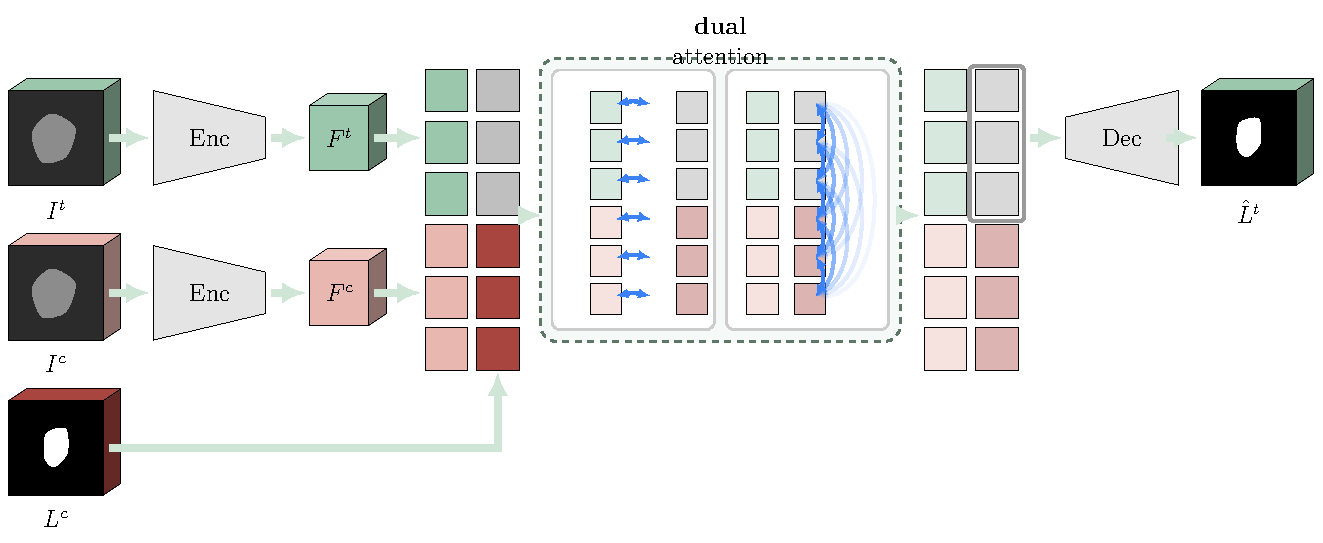
\includegraphics[width=\linewidth]{arch_patchset.pdf}
  \caption{Overview of the model at one cascade level. Target and context
  images pass through a shared encoder; image and label tokens are processed
  by dual attention; a decoder produces the target mask.}
  \label{fig:overview}
\end{figure}
\todo{Draft diagram, ported from the conference draft; finalize labels/scale once the architecture is settled.}

\paragraph{Shared encoder.}
All $K+1$ images of a task pass through the same encoder, a plain
convolutional encoder in the style of nnU-Net~\cite{isensee2021nnu} with four
stages, trained from scratch with He initialization. The encoder sees only
images; masks enter the model through the label tokens described below. The
first two stages (0 and 1) are the fine stages: they keep their own resolution
and serve as skip connections for the decoder
(\autoref{sec:methodology-fusion}). The last two stages (2 and 3) are the
coarse stages. Their features are resampled to a common grid of
$R \times R \times R$ cells with $R = 16$, giving $N = R^3 = 4096$ cells per
volume, and concatenated along the channel dimension. Each cell therefore
covers $p^3 = 8^3$ voxels of the input grid, with $p = 128/R$. The attention
layers always operate on this fixed grid, while the decoder can still produce
a mask at the full $128^3$ resolution.
\todo[inline]{\autoref{sec:results-fusion} says the fusion arms warm-start the
encoder and decoder from a shared checkpoint. Is that a checkpoint of this
model, itself trained from scratch? If so, say so there.}

\paragraph{Tokens.}
Each cell $i$ of each volume $v$ is represented by two tokens of dimension
$D = 768$. The image token is a linear projection of the concatenated coarse
features at that cell,
%
\begin{equation}
  z^{\text{img}}_{v,i} = W_{\text{img}} \, f_{v,i},
  \label{eq:img-token}
\end{equation}
%
where $f_{v,i}$ denotes the resampled stage-2 and stage-3 features of cell $i$.
The label token embeds the part of the mask that falls into the cell. We
flatten the $p^3 = 512$ mask voxels of cell $i$ into a vector $m_{v,i}$ and
project it linearly:
%
\begin{equation}
  z^{\text{lbl}}_{v,i} = \mathrm{LblEmbed}(m_{v,i}) = W_{\text{lbl}} \, m_{v,i} + b_{\text{lbl}}.
  \label{eq:lbl-token}
\end{equation}
%
For a context volume, $m_{v,i}$ is taken from the ground-truth mask $L^c_k$.
For the target, the mask is unknown. At the first cascade level, every target
cell receives the same placeholder: the average of $m_{v,i}$ over all cells of
all context volumes, embedded with $\mathrm{LblEmbed}$. It carries the average
amount of foreground in the context masks, but no information about where the
target is. At later levels, the target's label tokens are computed from the
previous level's prediction instead (\autoref{sec:methodology-cascade}).

Learned embeddings mark each token as belonging to the target or to a context
volume. Eight learned register tokens, shared across all volumes, are
prepended to the sequence. They are not tied to any cell and give the
attention layers a fixed amount of global memory.
% <<< end sections/methodology_overview.tex
% >>> begin sections/methodology_fusion.tex
% >>> begin sections/methodology_fusion.tex
\subsection{Dual Attention}\label{sec:methodology-fusion}

The attention layers have two jobs: combining image and label information, and
matching the target against the context. In Medverse and Iris, these happen at
fixed points in the network (\autoref{sec:fundamentals-relatedwork}).
\autoref{fig:fusion-family} contrasts Medverse's design with the
shared-encoder design used in this thesis.

\begin{figure}[t]
  \centering
  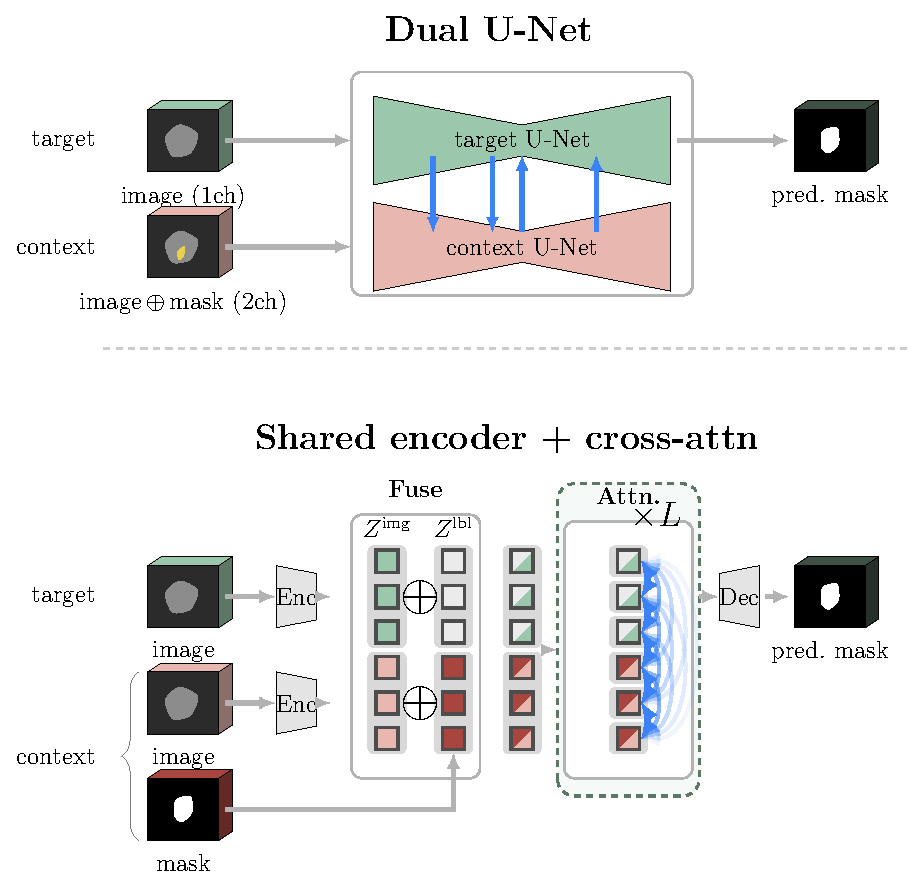
\includegraphics[width=\linewidth]{arch_fusion_family.pdf}
  \caption{Two ways of coupling target and context, shown for one context
  volume ($K{=}1$) and three of its $N$ tokens. Top: Medverse feeds the target
  image, and the context image and mask concatenated as channels, into two
  separate U-Nets that exchange features through cross-attention at several
  stages (blue arrows). Bottom: the shared-encoder design used in this thesis.
  Only images pass through the encoder. Label information is added to the
  encoded tokens afterwards, the tokens attend across cells and volumes for
  $L$ layers, and a shared decoder produces the mask. \autoref{fig:fusion-axis}
  shows the two ways of adding label information that we compare.}
  \label{fig:fusion-family}
\end{figure}
\todo{Draft diagram, ported from the conference draft; finalize once the layer factorization is settled.}

\paragraph{Token array.}
We arrange all tokens of a task in an array
$Z \in \mathbb{R}^{S \times 2 \times D}$. Each of its $S$ rows corresponds to
one cell of one volume or to one register token, and its two columns hold the
image stream and the label stream (\autoref{sec:methodology-overview}). With
$K+1$ volumes of $N$ cells and eight registers, $S = (K+1)N + 8$. Dual attention attends along
each of the two axes of this array in turn, following the general pattern of
the dual attention network of Fu et al.~\cite{fuDualAttentionNetwork2019},
which combines position-wise and channel-wise attention for scene
segmentation.
\todo[inline]{Confirm: register and pooling rows also have an entry in both
streams (implied by the $c{=}2$ layout). How are they initialized in the label
stream?}

\paragraph{Layer structure.}
Each of the $L = 4$ layers applies three residual blocks, each preceded by
RMS normalization:
%
\begin{align}
  Z &\leftarrow Z + \mathrm{Attn}_{\text{mod}}\big(\mathrm{RMSNorm}_1(Z)\big), \\
  Z &\leftarrow Z + \mathrm{Attn}_{\text{pos}}\big(\mathrm{RMSNorm}_2(Z)\big), \\
  Z &\leftarrow Z + \mathrm{MLP}\big(\mathrm{RMSNorm}_3(Z)\big).
  \label{eq:dual-layer}
\end{align}
%
\begin{itemize}[leftmargin=1.4em,itemsep=0.1em]
  \item \textbf{Modality axis} ($\mathrm{Attn}_{\text{mod}}$). Within each
    row, the image token and the label token attend to each other. This is
    attention over a sequence of length two, computed independently for every
    row, so its cost grows linearly with $S$.
  \item \textbf{Position axis} ($\mathrm{Attn}_{\text{pos}}$). Within each
    stream, the tokens of all rows attend to each other: image tokens attend
    to the image tokens of all cells, volumes, and registers, and label tokens
    likewise to label tokens. The two streams use the same attention weights
    but are processed as separate sequences of length $S$. Attention is
    unmasked, so every row attends to every other row, including context rows
    to target rows and vice versa. Queries and keys use 3D axial RoPE with
    physical coordinates (\autoref{sec:fundamentals-backbone}), so attention
    depends on the physical distance between cells. The cost grows
    quadratically with $S$.
  \item \textbf{MLP}. Two linear layers with a GELU activation in between,
    applied to each token independently, with hidden dimension 3072.
\end{itemize}
%
All attention operations use 12 heads with a token dimension of $D = 768$.
\todo[inline]{Confirm: (1) the position axis shares its weights between the
two streams (implied by batching the streams into the batch dimension);
(2) how RoPE is applied to register and pooling rows, which have no spatial
position.}

The two streams exchange information only in the modality axis, which is local
to a cell. Matching across cells and volumes happens within each stream.
Because the modality axis comes first in every layer, the tokens entering the
position axis already combine image and label information of their cell, so
both streams can use both kinds of information when matching across cells.
Since attention is unmasked, the context tokens also depend on the target:
the context is encoded anew for each target, rather than once per task as in
Iris.

\paragraph{Early-fusion baseline.}
As a baseline, the early-fusion variant (\autoref{fig:fusion-axis}, top)
merges the image and label token of each cell into a single token before the
attention layers, using a pixel shuffle--unshuffle operation similar to the one
Iris uses in its context encoder. The array then has a single column, and each
layer applies only the position axis and the MLP. The image and label
information of a cell is thus combined once, before any attention, rather than
in every layer. Without the modality axis and the second stream, a layer costs
roughly half as much, so this variant uses $L = 9$ layers to match the compute
of dual attention (\autoref{sec:results-fusion}).
\todo[inline]{Describe the merge precisely: is the $8^3$ mask patch unshuffled
into channels and concatenated with the coarse features before the projection
$W_{\text{img}}$? Otherwise the same block structure (RMSNorm, MLP, 12 heads)?}

\begin{figure}[t]
  \centering
  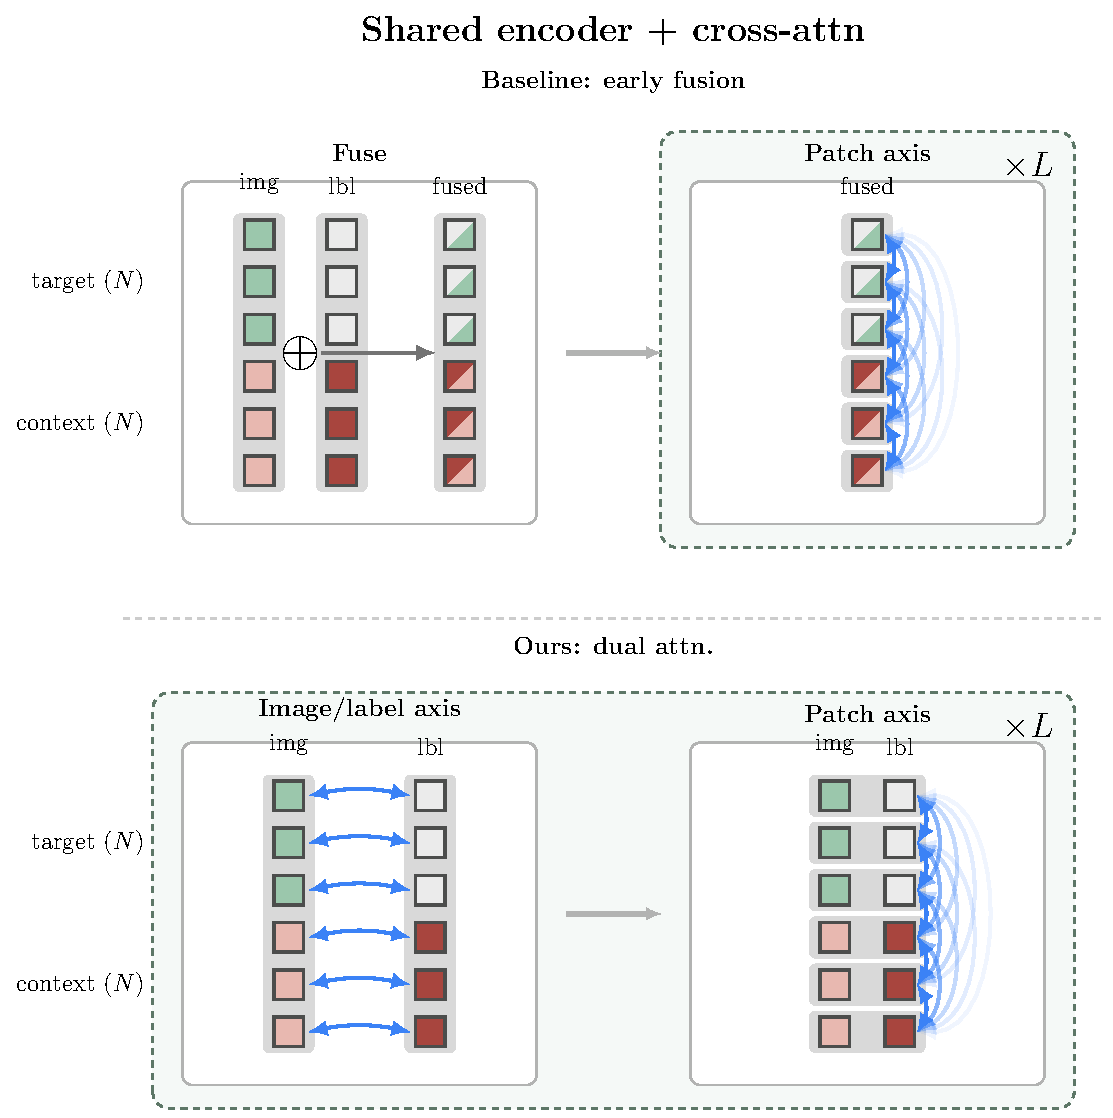
\includegraphics[width=\linewidth]{arch_fusion_axis.pdf}
  \caption{The two variants of the shared-encoder design compared in
  \autoref{sec:results-fusion}, shown for one context volume and three of its
  $N$ cells. Top: early fusion (baseline). Image and label tokens are merged
  once ($\oplus$), and the fused tokens attend across cells and volumes for
  $L$ layers. Bottom: dual attention. Image and label tokens stay in separate
  streams. In each of the $L$ layers, the two tokens of a cell attend to each
  other (modality axis), and then each stream attends across all cells and
  volumes (position axis). The target's label token (gray) holds the prior of
  \autoref{sec:methodology-cascade}, not ground truth.}
  \label{fig:fusion-axis}
\end{figure}
\todo{Draft diagram, ported from the conference draft; finalize once the layer factorization is settled. The position-axis panel should show two separate attentions, one per stream, not one joint attention over image and label tokens.}

% <<< end sections/methodology_fusion.tex% <<< end sections/methodology_fusion.tex
% >>> begin sections/methodology_cascade.tex
\subsection{Coarse-to-Fine Cascade}\label{sec:methodology-cascade}

Each of the $M$ levels processes a single $128^3$ crop; levels differ only in
spacing and hence field of view. The prediction of one level determines where
the next crop is placed and initializes the target's label tokens.

\paragraph{Crop placement.}
The first crop is centered at the center of the volume, with a spacing chosen
per dataset to cover the region where the target can occur. Each later crop
is centered at the probability-weighted centroid of the previous prediction,
or at the volume center if that prediction is empty. The finest spacing is
chosen so that the field of view exceeds the largest expected target
(\autoref{tab:cascade-levels}). Each level thus costs one forward pass,
independent of volume and target size. We refer to this as region
restriction. Its drawbacks are that a target missed at a coarse level cannot
be recovered, and that a target with several distant components may not fit
into one fine crop.

\paragraph{Stitching.}
The coarsest prediction is pasted into the original volume first; each finer
level then overwrites the region covered by its crop.

\paragraph{Prediction as prior.}
At level $\ell > 1$, the target's label tokens are computed from the previous
prediction, cell by cell as in \autoref{eq:lbl-token}:
%
\begin{equation}
  z^{\text{lbl}}_{\ell,0} = \mathrm{LblEmbed}\big(\mathrm{Warp}_{\ell-1 \to \ell}(\hat{L}^t_{\ell-1})\big),
  \label{eq:query-prior}
\end{equation}
%
where $\hat{L}^t_{\ell-1}$ is the sigmoid probability map of level $\ell{-}1$,
detached from the computation graph, and $\mathrm{Warp}$ resamples it onto the
crop grid of level $\ell$. The prior thus enters the same stream as the
context masks, instead of a separate branch as in Medverse
(\autoref{sec:fundamentals-relatedwork}); see \autoref{fig:query-prior}.

\begin{figure}[t]
  \centering
  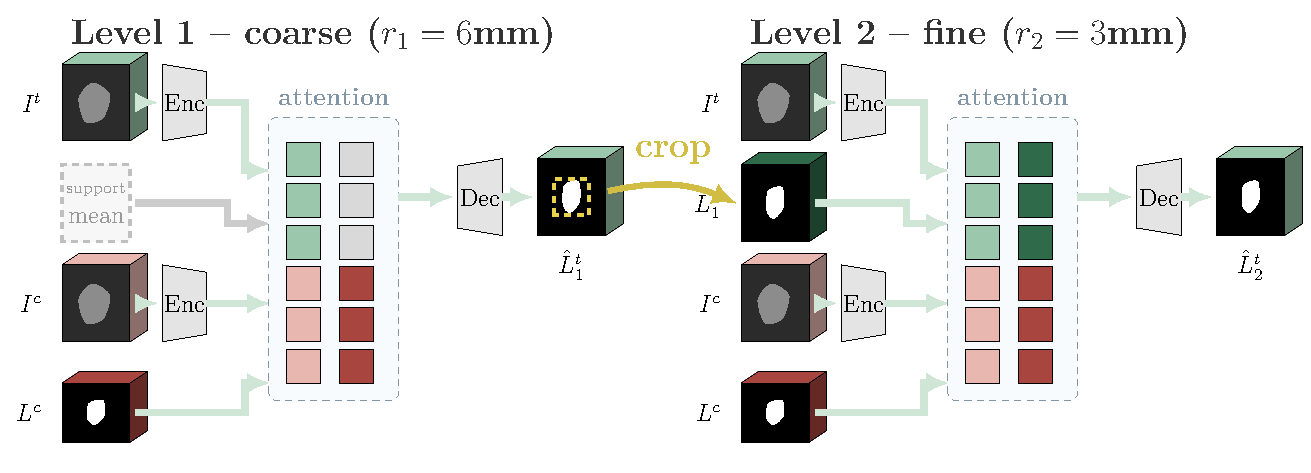
\includegraphics[width=\linewidth]{arch_query_prior.pdf}
  \caption{Label prior across two cascade levels. At level 1, the target's
  label tokens hold a placeholder (dashed); at level 2, a crop of the level-1
  prediction $\hat{L}^t_1$.}
  \label{fig:query-prior}
\end{figure}
\todo{Draft diagram, ported from the conference draft; finalize once the number of levels $M$ is settled.}

\paragraph{Training.}
All $M$ levels are processed in one forward pass. The first crop is centered
on the ground truth (at inference: on the volume center), later crops on the
previous prediction, at its centroid or at a random foreground point. The
coarsest spacing is drawn per batch, and each finer spacing log-uniformly
between the previous spacing and a lower bound, with a minimum ratio between
levels. The prior is either the model's own prediction (predicted prior) or
the ground truth, dilated or eroded, shifted, and with added Gaussian noise
(perturbed ground-truth prior); \autoref{sec:results-cascade} compares both.
\todo[inline]{Values: $M$, spacing range, lower bound, minimum ratio,
centroid vs.\ random-point probability, foreground threshold, perturbation
magnitudes. Confirm inference always uses the centroid.}% <<< end sections/methodology_cascade.tex
% >>> begin sections/methodology_synth.tex
% >>> begin sections/methodology_synth.tex
\subsection{Synthetic Task Generation}\label{sec:methodology-synth}

During training, a fraction $p_{\text{synth}}$ of tasks is generated
synthetically. For each synthetic task, one shape family and one set of shape
and appearance parameters are drawn; these play the role of the class. Each of
the $K+1$ volumes then receives its own instance of the shape, painted onto its
own image. Shape, size, and position vary between volumes with ratios of 0.3,
0.3, and 0.5, where 0 reuses the task-level value and 1 draws it
independently.

\paragraph{Shapes.}
Masks come from seven procedural families (\autoref{tab:synth-shapes}). The
scatter field places many small components across a region to imitate
multi-focal lesions, which few structures in the training cohort resemble.
Sizes are defined in millimeters and converted to voxels at each cascade
level, so a shape is the same physical object at every level.

\begin{table}[t]
  \centering
  \small
  \caption{Shape families. Target diameters are drawn from 10--50\,mm unless
  stated otherwise.}
  \label{tab:synth-shapes}
  \begin{tabular}{@{}ll@{}}
    \toprule
    Family & Family-specific parameters \\
    \midrule
    Blob, disk      & -- \\
    Splatter        & 2--6 components, spread 5--20\,mm \\
    Scatter field   & 10--120 components, spread 20--140\,mm \\
    Cylinder        & length 30--100\,mm \\
    Vessel          & trunk 40--120\,mm, branching depth 2--4 \\
    Torus           & ratio of major to minor radius 2--5 \\
    \bottomrule
  \end{tabular}
\end{table}

\paragraph{Canvas.}
We compare two sources for the images.
The \emph{real-host} canvas uses real TotalSegmentator scans. A host structure
is drawn, and $K+1$ different subjects containing it are sampled; the shape is
placed within $\pm 30$\,mm per axis of the host structure's centroid. Since the
volumes of a task are different scans, the target cannot be found by comparing
it with the context images voxel by voxel.
The \emph{synthetic-bank} canvas uses a bank of label maps from segmented CT
scans of about 21 datasets. A class is drawn, and $K+1$ label maps containing
it are selected, optionally preferring maps of similar geometry. As in
SynthSeg~\cite{billot2023synthseg}, the image is synthesized from the label
map with Gaussian-mixture intensities, and the shape is painted into it, with
an optional blend of core and rim intensity. Only the anatomical layout of this
canvas is real; its appearance is synthetic.

\paragraph{Appearance on the real-host canvas.}
The shape is painted relative to the local tissue statistics $\mu$ and
$\sigma$ of the host image:
%
\begin{equation}
  I(x) = \mu + c\,\sigma + \sigma\, n(x), \qquad c \sim \mathcal{U}(-2.5, 2.5),
  \label{eq:paint}
\end{equation}
%
with the contrast $c$ drawn once per task. The range covers the
lesion-to-tissue contrast we measured on seven of the evaluation datasets
(10th to 90th percentile: $-0.87$ to $2.00$), widened symmetrically because
the sign of the contrast is not known for an arbitrary host. The texture
$n(x)$ is fractal value noise with unit variance: four octaves of random grids,
starting from 15\,mm cells and halving the cell size per octave, weighted by
$0.5^k$.
\todo[inline]{Over which region are $\mu$ and $\sigma$ computed (a ring
around the shape?) Which seven datasets were used for the contrast
calibration?}
% <<< end sections/methodology_synth.tex% <<< end sections/methodology_synth.tex
% >>> begin sections/methodology_objective.tex
\subsection{Training Objective}\label{sec:methodology-objective}

Each cascade level is supervised at its own resolution with the sum of a
binary cross-entropy and a soft Dice loss:
%
\begin{equation}
  \mathcal{L} = \sum_{\ell=1}^{M} \lambda_\ell \left( \mathcal{L}_{\text{BCE}}^\ell + \mathcal{L}_{\text{Dice}}^\ell \right),
  \label{eq:loss}
\end{equation}
%
with uniform weights $\lambda_\ell = 1$. Because the prior is detached
(\autoref{sec:methodology-cascade}), the loss at level $\ell$ does not
propagate into level $\ell{-}1$. The single-level experiments of
\autoref{sec:results-fusion} use $M = 1$.% <<< end sections/methodology_objective.tex
% <<< end sections/methodology.tex
% >>> begin sections/results.tex
\section{\iflanguage{english}{Results}{Ergebnisse}}\label{sec:results}

% >>> begin sections/results_setup.tex
\subsection{Experimental Setup}\label{sec:results-setup}

\paragraph{Training data.}
Models are trained on the CT part of
TotalSegmentator~\cite{wasserthalTotalSegmentatorRobustSegmentation2023}
(1082 training, 57 validation, and 89 test subjects) and, except in
\autoref{sec:results-fusion}, on the TotalSegmentator MRI release~\cite{dantonoliTotalSegmentatorMRIRobust2025}
(561 training subjects from University Hospital Basel and the NIH Imaging
Data Commons). Training uses 61 of the 117 classes, chosen to balance
anatomical categories and structure thickness: 12 abdominal and pelvic organs,
8 thoracic, head, and spinal organs, 5 muscles (one side of each pair), 6 limb,
shoulder, and pelvic bones, 11 vertebrae spanning all spine regions, 9 ribs
and sternal structures, and 10 vessels. The remaining 56 classes form the
unseen split. (\autoref{tab:totalseg-classes}) It includes structures close to training classes, such as the
contralateral side of each training muscle. On MRI, 31 of the 61 training
classes are available.

\paragraph{Model configurations.}
The experiments were run at different stages of development, so the three
results sections use different model configurations
(\autoref{tab:configs}). Numbers from different sections are therefore not
directly comparable. In particular, TotalSegmentator MRI is a held-out
modality for the fusion experiments, which train on CT only, but part of the
training data in the other two sections.

\begin{table}[t]
  \centering
  \small
  \caption{Model configurations used in the results sections.}
  \label{tab:configs}
  \begin{tabular}{@{}lllll@{}}
    \toprule
    Name & Section & Training data & Levels & $p_\text{synth}$  \\
    \midrule
    Fusion arms & \ref{sec:results-fusion} & TotalSeg CT & 1 & 0  \\
    Cascade & \ref{sec:results-cascade}, \ref{sec:results-synth} & TotalSeg CT + MRI & 2--3 & 0 \\
    Synth & \ref{sec:results-synth} & TotalSeg CT + MRI & 1 & 0.5 \\
    Synth + Cascade & \ref{sec:results-synth} & TotalSeg CT + MRI & 2--3 & 0.5 \\
    \bottomrule
  \end{tabular}
\end{table}
\todo[inline]{Resolve before submission: report a single final configuration,
or keep this split?}

\paragraph{Baselines.}
The external baseline is Medverse~\cite{huMedverseUniversalModel2025a} with
its released weights (\autoref{sec:results-cascade},
\autoref{sec:results-synth}). In \autoref{sec:results-fusion}, we additionally
train Medverse's architecture from its released weights with our training
recipe.
\todo[inline]{No Iris baseline exists yet; the comparison in
\autoref{sec:fundamentals-relatedwork} remains architectural, not empirical.}

\paragraph{Evaluation protocol.}
Each target is segmented with a single context pair ($K = 1$). The context
subject is drawn at random, with a fixed seed per target, from the same dataset
and split as the target, among the subjects that contain the target class.
Every subject that contains a class serves once as a target for that class. For each model, we use the checkpoint with the best
Dice on the in-distribution validation split; no evaluation dataset is used for
checkpoint selection.
\todo[inline]{See open points: MRI validation split, $n$ in
\autoref{tab:ood-sources}, $K$ during training.}


\paragraph{Metrics.}
Accuracy is reported as Dice, computed per class and averaged over classes
unless stated otherwise, and as Normalized Surface Dice (NSD) with a tolerance
of 3\,mm. Compute is reported as GFLOPs per forward pass and as latency per
sample. All training and evaluation runs on a single NVIDIA
RTX PRO 6000 Blackwell Server Edition GPU (96\,GB).
\todo[inline]{Precision of the latency measurements in
\autoref{tab:cascade-medverse} (fp32 as in \autoref{tab:fusion-staircase}?).}

\paragraph{Datasets.}
\autoref{tab:ood-sources} lists the evaluation datasets, grouped by their
relation to the training classes. TotalSegmentator and FLARE22 contain classes
from the TotalSegmentator vocabulary, so their classes split into seen and
unseen ones. The other datasets contain targets that do not occur in training:
new anatomical structures, lesions, a measurement region that is not an
anatomical object, and, for the fusion experiments, an unseen modality.
Because of this split, "held-out" is used at two levels below: at the
dataset level (a dataset whose images were never trained on, e.g.\ FLARE22,
whose classes are nonetheless mostly in-vocabulary) and, where stated
explicitly as such, at the class level (excluding classes that are in the
training vocabulary, even if their dataset is held out).

\begin{table}[t]
  \centering
  \small
  \caption{Evaluation datasets, grouped by relation to the training classes.
  $n$: number of subjects; $n_\text{cls}$: number of evaluated classes.}
  \label{tab:ood-sources}
  \begin{tabular}{@{}lllll@{}}
    \toprule
    Dataset & Modality & Target & $n$ & $n_\text{cls}$ (seen/unseen) \\
    \midrule
    \multicolumn{5}{@{}l}{\itshape Training vocabulary (seen and unseen classes)} \\
    TotalSegmentator~\cite{wasserthalTotalSegmentatorRobustSegmentation2023} & CT &  full-body 
    anatomical structures & 89 & 117 (61/56) \\
    FLARE22~\cite{maFLARE22Challenge2024} & CT & abdominal organs & 50 & 13 (11/2) \\
    \midrule
    \multicolumn{5}{@{}l}{\itshape New targets} \\
    ISLES22~\cite{hernandezpetzscheIsles2022Multicenter2022} & MRI DWI & stroke lesion & 250 & 1 \\
    Shifts-MS~\cite{malininShifts20Extending2022} & MRI FLAIR & MS lesions & 46 & 1 \\
    MSD Hippocampus~\cite{antonelliMedicalSegmentationDecathlon2022} & MRI T1 & hippocampus & 260 & 2 \\
    MSD Prostate~\cite{antonelliMedicalSegmentationDecathlon2022} & MRI T2 + ADC & prostate zones & 64 & 2 \\
    ATLAS v2.0$^{*}$~\cite{liewLargeCuratedOpensource2022} & MRI T1 & chronic stroke lesion & 654 & 1 \\
    GNC\_705 & MRI Dixon & kidney lesions & 610 & 13 \\
    NasalSeg~\cite{zhangNasalSegDataset2024} & CT & nasal cavity and sinuses & 107 & 5 \\
    \midrule
    \multicolumn{5}{@{}l}{\itshape Non-anatomical target} \\
    HU\_LWK1 & CT & center of L1 vertebrae & 36 & 1 \\
    \midrule
    \multicolumn{5}{@{}l}{\itshape Additional modality (unseen in \autoref{sec:results-fusion})} \\
    TotalSeg MRI~\cite{dantonoliTotalSegmentatorMRIRobust2025} & MRI & full-body 
    anatomical structures & 47 & 50 (31/19) \\
    \bottomrule
  \end{tabular}
  \par\vspace{0.5em}
  \raggedright\footnotesize
  $^{*}$Obtained from an unofficial mirror; provenance not yet confirmed.
\end{table}
% <<< end sections/results_setup.tex
% >>> begin sections/results_fusion.tex
\subsection{Image--Label Fusion}\label{sec:results-fusion}

This section compares three architectures. The comparison between Dual U-Net
Cross-Attn and early fusion tests the change from two U-Nets coupled by
cross-attention to a shared encoder with attention layers. The comparison
between early fusion and dual attention tests whether, within the
shared-encoder design, keeping image and label tokens separate improves over
merging them once.

\paragraph{Architectures.}
\emph{Dual U-Net Cross-Attn} is Medverse's architecture
(\autoref{sec:fundamentals-relatedwork}), initialized from the released weights
and then trained with our recipe. It is therefore a different model from the
released Medverse baseline used in \autoref{sec:results-cascade}.
\emph{Early fusion} and \emph{dual attention} are the two variants shown in
\autoref{fig:fusion-axis}. Early fusion uses $L{=}9$ layers to match the compute of dual attention (\autoref{sec:methodology-fusion}).
This gives both variants similar compute (3973 vs.\ 3892 GFLOPs). Parameter
count could not be matched at the same time, and early fusion has 52\% more
parameters. Dual U-Net Cross-Attn is not compute-matched to either variant.

\paragraph{Training.}
All three architectures use the same training recipe
(\autoref{tab:fusion-trainsettings}), data pipeline, and augmentations. They
are trained on the CT cases and training classes of TotalSegmentator, without
synthetic tasks, at a single level. Their initialization differs. Dual U-Net
Cross-Attn starts from Medverse's weights. Early fusion and dual attention
are randomly initialized. Dual U-Net Cross-Attn completed its training
budget; early fusion and dual attention were stopped before completing
theirs, so the comparison also reflects this difference in training progress,
not only initialization.

\begin{table}[t]
  \centering
  \small
  \caption{Training settings shared by the three architectures of
  \autoref{sec:results-fusion}.}
  \label{tab:fusion-trainsettings}
  \begin{tabular}{@{}ll@{}}
    \toprule
    Optimizer & AdamW \\
    Learning rate & $10^{-4}$ \\
    Schedule & cosine decay, 10-epoch warmup \\
    Weight decay & $10^{-2}$ \\
    Batch size & 8 \\
    Gradient clipping & 1.0 \\
    Loss & BCE + Dice \\
    Epochs & 250 \\
    \bottomrule
  \end{tabular}
\end{table}

\paragraph{Evaluation.}
All three architectures are evaluated at a single level with 3\,mm spacing, in
fp32, using the best checkpoint of each.
\autoref{tab:fusion-staircase} reports the results, grouped as in
\autoref{tab:ood-sources}.
\todo[inline]{Specify where the 3\,mm crops are placed (centered on the ground
truth?).}

\begin{table}[t]
  \centering
  \small
  \caption{Dice of the three architectures at a single level (3\,mm), with
  parameter count, compute, and latency.}
  \label{tab:fusion-staircase}
  \begin{tabular}{@{}lccc@{}}
    \toprule
    & Dual U-Net Cross-Attn & Early fusion & Dual attention \\
    \midrule
    TotalSeg CT, seen      & 0.348 & 0.574 & \textbf{0.582} \\
    TotalSeg CT, unseen    & 0.221 & 0.408 & \textbf{0.426} \\
    FLARE22, seen          & 0.532 & 0.693 & \textbf{0.709} \\
    FLARE22, unseen        & 0.443 & \textbf{0.632} & 0.604 \\
    \midrule
    MSD Prostate           & \textbf{0.377} & 0.205 & 0.247 \\
    MSD Hippocampus        & 0.172 & 0.122 & \textbf{0.184} \\
    \midrule
    HU\_LWK1               & \textbf{0.146} & 0.079 & 0.102 \\
    \midrule
    TotalSeg MRI           & 0.178 & 0.232 & \textbf{0.259} \\
    \midrule
    ISLES22                & \textbf{0.046} & 0.037 & 0.043 \\
    Shifts-MS               & 0.087 & 0.038 & \textbf{0.109} \\
    ATLAS v2.0              & \textbf{0.031} & 0.014 & 0.022 \\
    GNC\_705                & \textbf{0.044} & 0.014 & 0.025 \\
    NasalSeg                & \textbf{0.434} & 0.272 & 0.358 \\
    \midrule
    Mean of 10 held-out sources$^{\dagger}$ & 0.187 & 0.174 & \textbf{0.201} \\
    \midrule
    Parameters             & 71.1M  & 74.1M  & 48.7M  \\
    GFLOPs                 & 2362.6 & 3973.1 & 3892.5 \\
    Latency per sample     & 73.2\,ms & 73.0\,ms & 72.5\,ms \\
    \bottomrule
  \end{tabular}
  \par\vspace{0.5em}
  \raggedright\footnotesize
  $^{\dagger}$MSD Prostate, MSD Hippocampus, HU\_LWK1, TotalSeg MRI, FLARE22
  (all 13 classes, not split by seen/unseen as above), ISLES22, Shifts-MS,
  ATLAS v2.0, GNC\_705, and NasalSeg — held-out at the dataset level
  (\autoref{sec:results-setup}). Sample-weighted: each dataset's macro Dice is
  weighted by its number of evaluated tasks (36 for HU\_LWK1 to 1490 for
  GNC\_705) rather than counted once per dataset, since task counts differ by
  up to $40\times$. The unweighted mean-of-datasets (0.203/0.170/0.204) and
  the fully pooled per-task mean (0.186/0.172/0.200) rank the three
  architectures identically.
\end{table}

\paragraph{Results.}
Early fusion outperforms Dual U-Net Cross-Attn on the classes from the
training vocabulary, by 0.16 to 0.23 Dice on TotalSegmentator and FLARE22, and
by a smaller margin on the unseen-modality TotalSeg MRI (0.232 vs.\ 0.178). It
is worse on the three sources with new or non-anatomical targets: MSD
Prostate, MSD Hippocampus, and HU\_LWK1.

Dual attention improves over early fusion on seven of the eight rows. The
gains are small on the other in-vocabulary rows (0.008 to 0.018) and larger on
the new targets and the unseen modality: MSD Hippocampus ($+0.062$), MSD
Prostate ($+0.042$), TotalSeg MRI ($+0.027$), and HU\_LWK1 ($+0.023$). The
exception is the unseen FLARE22 classes, where dual attention scores 0.028
lower.

Compared with Dual U-Net Cross-Attn, dual attention is better on six of the
eight rows, including MSD Hippocampus (0.184 vs.\ 0.172), but remains worse on
MSD Prostate (0.247 vs.\ 0.377) and HU\_LWK1 (0.102 vs.\ 0.146).

On the five lesion and cavity datasets in \autoref{tab:fusion-staircase}
(ISLES22, Shifts-MS, ATLAS v2.0, GNC\_705, NasalSeg), the pattern reverses:
Dual U-Net Cross-Attn is best of the three on four of five, losing only on
Shifts-MS, where dual attention is best (0.109 vs.\ 0.087). Dual attention's
margin behind Dual U-Net Cross-Attn on the other four is at most 0.076
(NasalSeg).

On the sample-weighted mean over all ten held-out sources, early fusion is
below Dual U-Net Cross-Attn (0.174 vs.\ 0.187), while dual attention is above
it (0.201); the unweighted mean-of-datasets and the fully pooled per-task mean
rank the three architectures the same way. This aggregate advantage for dual
attention comes from the first five sources, not the lesion and cavity ones,
where Dual U-Net Cross-Attn wins more often. The shared-encoder design alone
thus improves accuracy on the training vocabulary, and dual attention improves
on held-out sources in aggregate, though not on every individual source.

Dual attention has the fewest parameters of the three (48.7M). Its compute is
similar to early fusion by construction and 65\% higher than Dual U-Net
Cross-Attn. Latency is nearly identical for all three (72.5 to 73.2\,ms)
despite these differences in GFLOPs.

% <<< end sections/results_fusion.tex
% >>> begin sections/results_cascade.tex
\subsection{Coarse-to-Fine Cascade}\label{sec:results-cascade}

This section evaluates the Cascade configuration (\autoref{tab:configs}). We
first examine how accuracy develops across levels and how well the coarse level
localizes the target. We then compare with Medverse in accuracy and latency,
and finally compare the two sources of the label prior.

\paragraph{Accuracy across levels.}
When the crop is centered on the ground truth, reducing the spacing from 4\,mm
to 1.5\,mm raises macro Dice on TotalSegmentator from 0.361 to 0.538 (117
classes, 3897 samples). Because these crops use the ground-truth position, this
shows the benefit of finer resolution, not of the cascade.
\autoref{tab:cascade-levels} therefore reports the Dice of each level when its
crop is placed using the previous level's prediction. Dice still increases from
level to level on every dataset, for example from 0.394 to 0.523 to 0.577 on
TotalSeg CT.
\todo[inline]{This shows that the cascade works without ground-truth
localization, but not that it beats a single fine-resolution pass over the
whole volume. The planned $-$region-restriction ablation answers this.}

\begin{table}[t]
  \centering
  \small
  \caption{Dice of the Cascade model at each level, with crops placed using the
  previous level's prediction, and Dice of the final stitched prediction.}
  \label{tab:cascade-levels}
  \begin{tabular}{@{}lccc@{}}
    \toprule
    Dataset & Spacings (mm) & Dice per level & Stitched \\
    \midrule
    TotalSeg CT  & $[6, 3, 1.5]$    & $0.394 \to 0.523 \to 0.577$ & 0.586 \\
    TotalSeg MRI & $[6, 3, 1.5]$    & $0.365 \to 0.481 \to 0.497$ & 0.506 \\
    HU\_LWK1     & $[6, 3, 1]$      & $0.065 \to 0.109 \to 0.152$ & 0.152 \\
    FLARE22      & $[6, 3, 2.5]$    & $0.603 \to 0.718 \to 0.751$ & 0.751 \\
    MSD Prostate & $[3, 1.5, 0.75]$ & $0.276 \to 0.361 \to 0.381$ & 0.375 \\
    NasalSeg     & $[1.5, 0.8]$     & $0.484 \to 0.547$           & 0.547 \\
    \bottomrule
  \end{tabular}
\end{table}

 Outside the finest crop, the stitched mask contains the predictions of
  coarser levels, so its Dice can be higher than the finest level's (TotalSeg
  CT and MRI), lower (MSD Prostate), or unchanged (HU\_LWK1, FLARE22,
  NasalSeg) when the target lies entirely inside the finest crop and there is
  nothing outside it for a coarser prediction to add.
  
\paragraph{Localization.}
  On TotalSeg CT (117 classes), at the coarsest level, the crop of the middle
  level, placed at the centroid of the coarse prediction, contains on average
  92.2\% of the target's voxels; placed at the ground-truth centroid, the same
  crop contains 97.0\%. Across classes, this
containment correlates only weakly with the Dice gain from the finer levels
($r = -0.22$, $p = 0.018$, $n = 117$, $r^2 \approx 0.05$). This measures only
the coarsest-to-middle transition, not the middle-to-finest one. Since most of
the target already lies inside the box at this first step, most of the
remaining error at this step arises within the fine crops rather than from
localization; whether the same holds for the middle-to-finest transition is
not tested here.

\paragraph{Comparison with Medverse.}
\autoref{tab:cascade-medverse} compares Cascade with Medverse's released
weights, using its own autoregressive coarse-to-fine inference. We report
Medverse both at its native number of refinement steps and with the number of
steps matched to our number of levels per dataset. Four lesion datasets
(ISLES22, Shifts-MS, ATLAS v2.0, GNC\_705), where both models score below 0.1,
appear at the bottom of the table with Cascade and Medverse's native depth
only: no step-matched Medverse run exists for them yet. MSD Hippocampus is
processed at a single level, so its row compares the base models without a
cascade.

\begin{table}[t]
  \centering
  \small
  \caption{Cascade vs.\ Medverse: macro Dice and mean latency per sample.
  Medverse is evaluated with its number of autoregressive steps matched to our
  number of levels (matched) and at its native number of steps (native).}
  \label{tab:cascade-medverse}
  \begin{tabular}{@{}lccccccc@{}}
    \toprule
    & & \multicolumn{3}{c}{Dice} & & \multicolumn{2}{c}{Latency (ms)} \\
    \cmidrule(lr){3-5} \cmidrule(lr){7-8}
    Dataset & Spacings (mm) & Cascade & \makecell{Medverse\\matched} & \makecell{Medverse\\native} & & Cascade & \makecell{Medverse\\matched} \\
    \midrule
    TotalSeg CT     & $[6, 3, 1.5]$    & \textbf{0.586} & 0.103 & --    & & 278 & 4978 \\
    FLARE22         & $[6, 3, 2.5]$    & \textbf{0.751} & 0.359 & 0.440 & & 311 & 4894 \\
    MSD Prostate    & $[3, 1.5, 0.75]$ & 0.375 & 0.357 & \textbf{0.423} & & 279 & 5006 \\
    MSD Hippocampus & $[0.5]$          & 0.303 & 0.686 & \textbf{0.691} & & 99  & 50   \\
    HU\_LWK1        & $[6, 3, 1]$      & \textbf{0.152} & 0.020 & 0.071 & & 439 & 5336 \\
    TotalSeg MRI    & $[6, 3, 1.5]$    & \textbf{0.506} & 0.038 & --    & & 306 & 4842 \\
    NasalSeg        & $[1.5, 0.8]$     & 0.547 & \textbf{0.737} & 0.735 & & 161 & 1886 \\
    \midrule
    Mean            &                  &       &       &       & & 268 & 3856 \\
    \midrule
    ISLES22         & $[3, 1.5]$       & \textbf{0.069} & -- & 0.053 & & 155 & -- \\
    Shifts-MS       & $[3, 1.5]$       & 0.031 & -- & \textbf{0.152} & & 289 & -- \\
    ATLAS v2.0      & $[3.8, 1.9]$     & \textbf{0.026} & -- & 0.023 & & 149 & -- \\
    GNC\_705        & $[6, 3, 1.2]$    & \textbf{0.024} & -- & 0.011 & & 288 & -- \\
    \bottomrule
  \end{tabular}
  \par\vspace{0.5em}
  \raggedright\footnotesize
  Mean is computed over the seven datasets above the second midrule, which
  have a step-matched Medverse run; the four lesion datasets below lack one.
\end{table}
\todo[inline]{Re-run TotalSeg CT with matched steps and measure its latency.
Add native runs for TotalSeg CT and MRI. Run a step-matched Medverse pass for
ISLES22/Shifts-MS/ATLAS v2.0/GNC\_705 to fill their ``--'' cells.
\texttt{\textbackslash makecell} needs the \texttt{makecell} package.}

Against Medverse with matched steps, Cascade is more accurate on five of the
seven datasets: TotalSeg CT, FLARE22, MSD Prostate, HU\_LWK1, and TotalSeg MRI.
Medverse is more accurate on MSD Hippocampus, reportedly part of its training
classes but not of ours, and on NasalSeg, which neither model saw during
training. Matching the number of steps lowers Medverse's accuracy on four of
the five datasets with a native run, most clearly on FLARE22 (0.440 to 0.359)
and HU\_LWK1 (0.071 to 0.020). Against Medverse at its native depth, Cascade
is more accurate on FLARE22 and HU\_LWK1 and less accurate on MSD Prostate,
MSD Hippocampus, and NasalSeg. On the four lesion datasets, which only have a
native comparison, Cascade is more accurate on three (ISLES22, ATLAS v2.0,
GNC\_705) and Medverse on one (Shifts-MS); all Dice values there are below
0.1 except Medverse's native Shifts-MS result (0.152).

\autoref{fig:cascade-medverse-qual} shows one case from each side of this
comparison, using the context, ground truth, and prediction of both models on
the same target subject (Medverse run in its native-autoregressive mode).
Ground truth is shown in green, Cascade's prediction in blue, Medverse's in
orange throughout this section. On FLARE22 gallbladder, Cascade recovers the
organ's shape (Dice 0.79) while Medverse predicts a small mislocated fragment
(Dice 0.00). On MSD Hippocampus, the pattern reverses: Cascade's prediction is
fragmented into disconnected blobs (Dice 0.34), while Medverse produces a
single contiguous region closer to the ground-truth shape (Dice 0.59).

\begin{figure}[t]
  \centering
  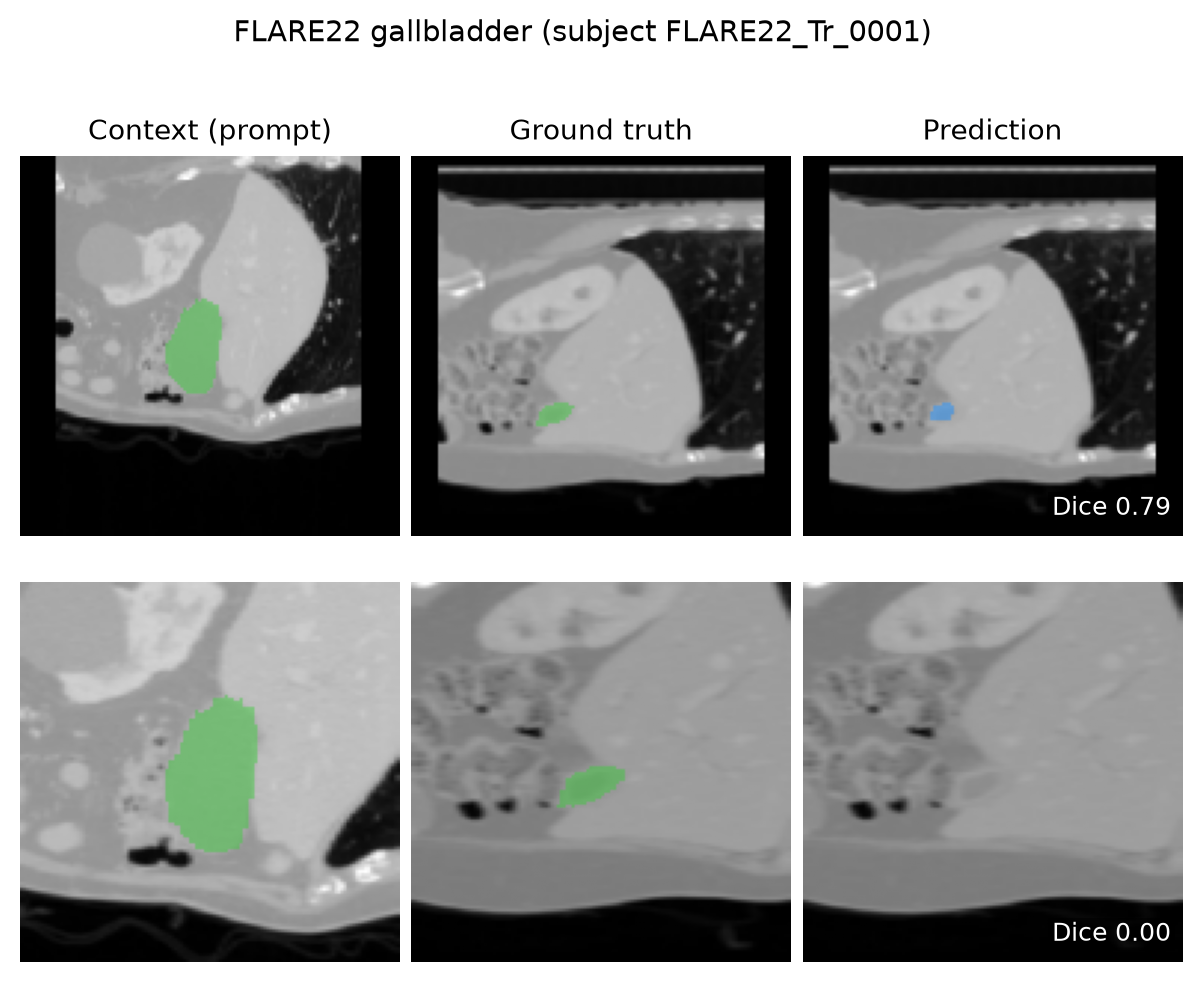
\includegraphics[width=0.85\linewidth]{flare22_gallbladder_win.png}
  \caption{FLARE22 gallbladder, subject FLARE22\_Tr\_0001: Cascade recovers
  the organ shape where Medverse's native-autoregressive prediction misses
  almost entirely.}
  \label{fig:cascade-medverse-qual}
\end{figure}

\begin{figure}[t]
  \centering
  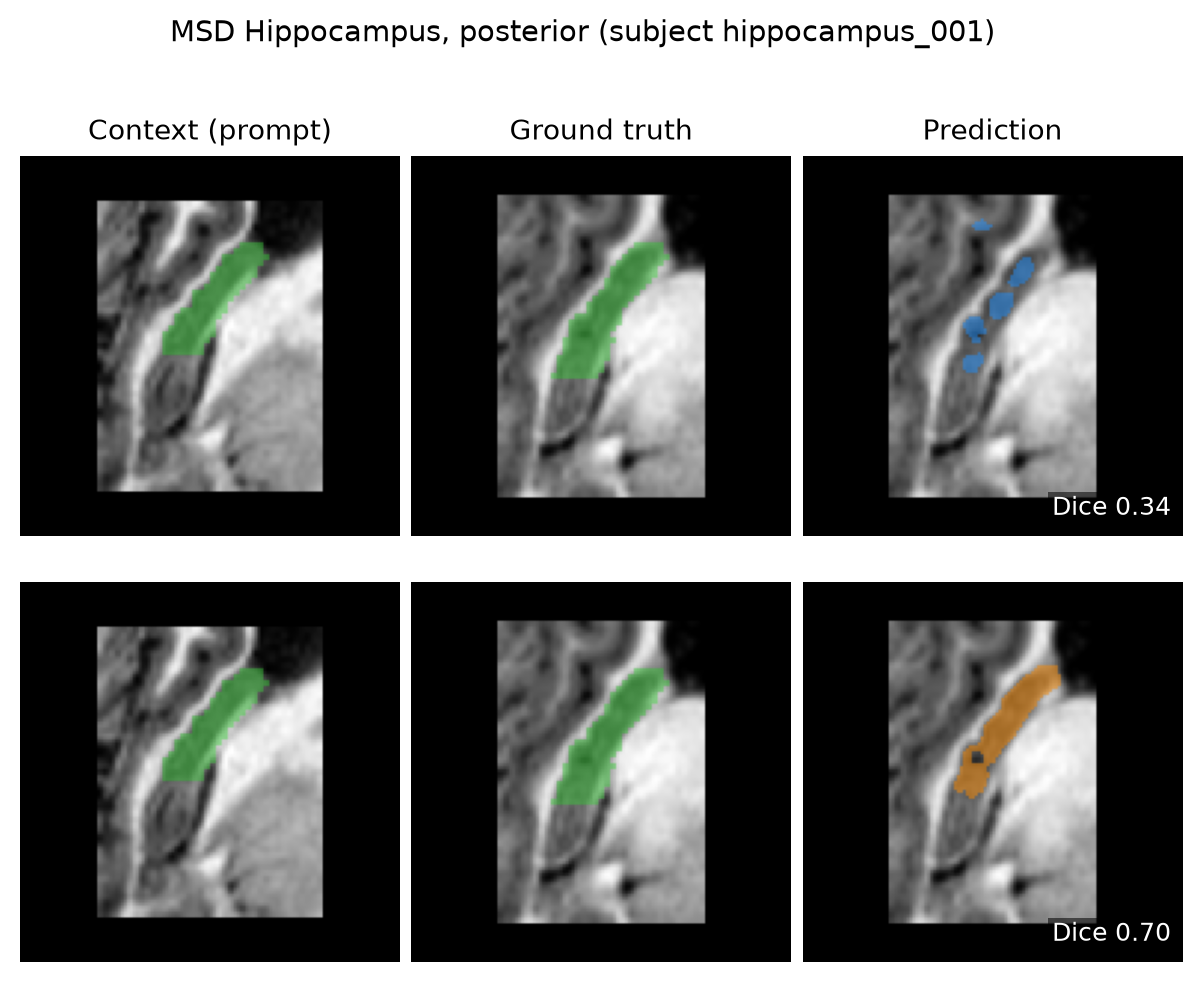
\includegraphics[width=0.85\linewidth]{msd_hippocampus_fail.png}
  \caption{MSD Hippocampus, posterior class, subject hippocampus\_001:
  Cascade's prediction fragments into disconnected blobs, while Medverse's
  native-autoregressive prediction stays a single contiguous region.}
  \label{fig:cascade-medverse-qual-fail}
\end{figure}
\todo[inline]{Both panels are re-rendered directly from run\_cascade /
model.predict() outputs on these two (target, context) pairs -- checkpoints
and settings matching
\texttt{2026-09-26\_147\_cascade\_randomfg\_predprior\_regon\_flare22\_ood} /
\texttt{2026-09-15\_medverse\_ar\_flare22} and
\texttt{2026-09-24\_146\_cascade\_randomfg\_predprior\_regoff\_msd\_hippocampus\_ood}
/ \texttt{2026-09-14\_medverse\_ar\_msd\_hippocampus} -- rather than the
harness's own saved diagnostic panels, so the color scheme could be made
consistent across models (green/blue/orange). Each sample is the first the
eval loader hit for its class, not a systematic best/worst search; Medverse's
native-AR dice on this MSD Hippocampus sample varies by a few hundredths
between runs (bf16-autocast nondeterminism), so treat 0.59 as approximate.}

Cascade is on average about $14\times$ faster than step-matched Medverse (268
vs.\ 3856\,ms per sample); excluding the estimated TotalSeg CT value gives a
similar ratio ($13.8\times$ vs.\ $14.4\times$ with it). Our model runs one forward pass per level, whereas Medverse slides a window over the whole volume at each step; this difference and the architectures are not separated here. On MSD
Hippocampus, where neither model uses a cascade, Medverse is faster (50 vs.\
99\,ms).

TotalSeg CT and MRI are part of our training data. The large differences on
these two rows therefore partly reflect training data, not only architecture.
\todo[inline]{State what Medverse was trained on, including whether MSD
Hippocampus is actually among its training classes (currently asserted above
without a citation) and whether its training data includes TotalSegmentator.
Its Dice of 0.103 on TotalSeg CT and 0.038 on TotalSeg MRI is very low; if
Medverse's training data includes TotalSegmentator, check preprocessing
(orientation, intensity normalization, spacing) before reporting these
numbers.}

\paragraph{Medverse with our cascade.}
We also ran Medverse's weights inside our cascade inference
(\autoref{sec:methodology-cascade}), with and without its coarse prediction
passed on as a prior, on these seven eval-expansion sources: HU\_LWK1,
ISLES22, Shifts-MS, MSD Hippocampus, MSD Prostate, ATLAS v2.0, and GNC\_705
(distinct from \autoref{tab:cascade-medverse}'s seven datasets, which instead
include TotalSeg CT, FLARE22, TotalSeg MRI, and NasalSeg). Each source uses
its own multi-level ladder, e.g.\ $[6,3,0.5]$\,mm for MSD Hippocampus; unlike
our own model, which runs MSD Hippocampus single-level in
\autoref{tab:cascade-medverse}, Medverse is given an actual cascade here on
every source, so the two MSD Hippocampus numbers come from different
evaluation setups. \autoref{tab:medverse-prior-appendix} in the appendix
reports the full results; passing the prior lowered Dice on six of the seven,
and on HU\_LWK1, Dice is 0.0 in both cases. The largest drop is on MSD
Hippocampus, from 0.691 to 0.050. Errors of Medverse's coarse prediction
therefore propagate strongly through its prior.

\autoref{fig:cascade-vs-medverse-cascade} shows two cases from this
comparison. To make the coarse-to-fine progression directly comparable, both
models are run on a common ladder for each figure (rather than each model's
own ladder from \autoref{tab:medverse-prior-appendix}, which differ in depth
and spacing), one column per shared physical spacing. On MSD Prostate TZ
(ladder $[6,3,1.5,0.75]$\,mm, common to both), Cascade's prediction grows to
fill the zone's shape across the four levels (Dice 0.69) while Medverse's box
tracks the same region but never produces a prediction at any level (Dice
0.00). On MSD Hippocampus (ladder $[6,3,0.5]$\,mm, common to both -- Cascade
is forced through this cascade here, whereas \autoref{tab:cascade-medverse}
runs it single-level), Medverse's box is again placed correctly at every
level but stays empty throughout (Dice 0.00), while Cascade's prediction
appears already at the coarsest level and refines into a fragmented but
non-empty final mask (Dice 0.43). This pattern is not universal:
\autoref{fig:cascade-vs-medverse-cascade-atlas} shows the clearest
counter-example found, an ATLAS v2.0 case (ladder $[6,3,1.9]$\,mm, common to
both -- Cascade normally runs $[3.8,1.9]$\,mm here) where Cascade's predicted
region shrinks to almost nothing by its finest level (Dice 0.01) while
Medverse's prior-conditioned prediction grows to cover much of the lesion
(Dice 0.42) -- well above ATLAS v2.0's aggregate Prior Dice of 0.020 in
\autoref{tab:medverse-prior-appendix}, so this single sample should not be
read as typical of that row.

\begin{figure}[t]
  \centering
  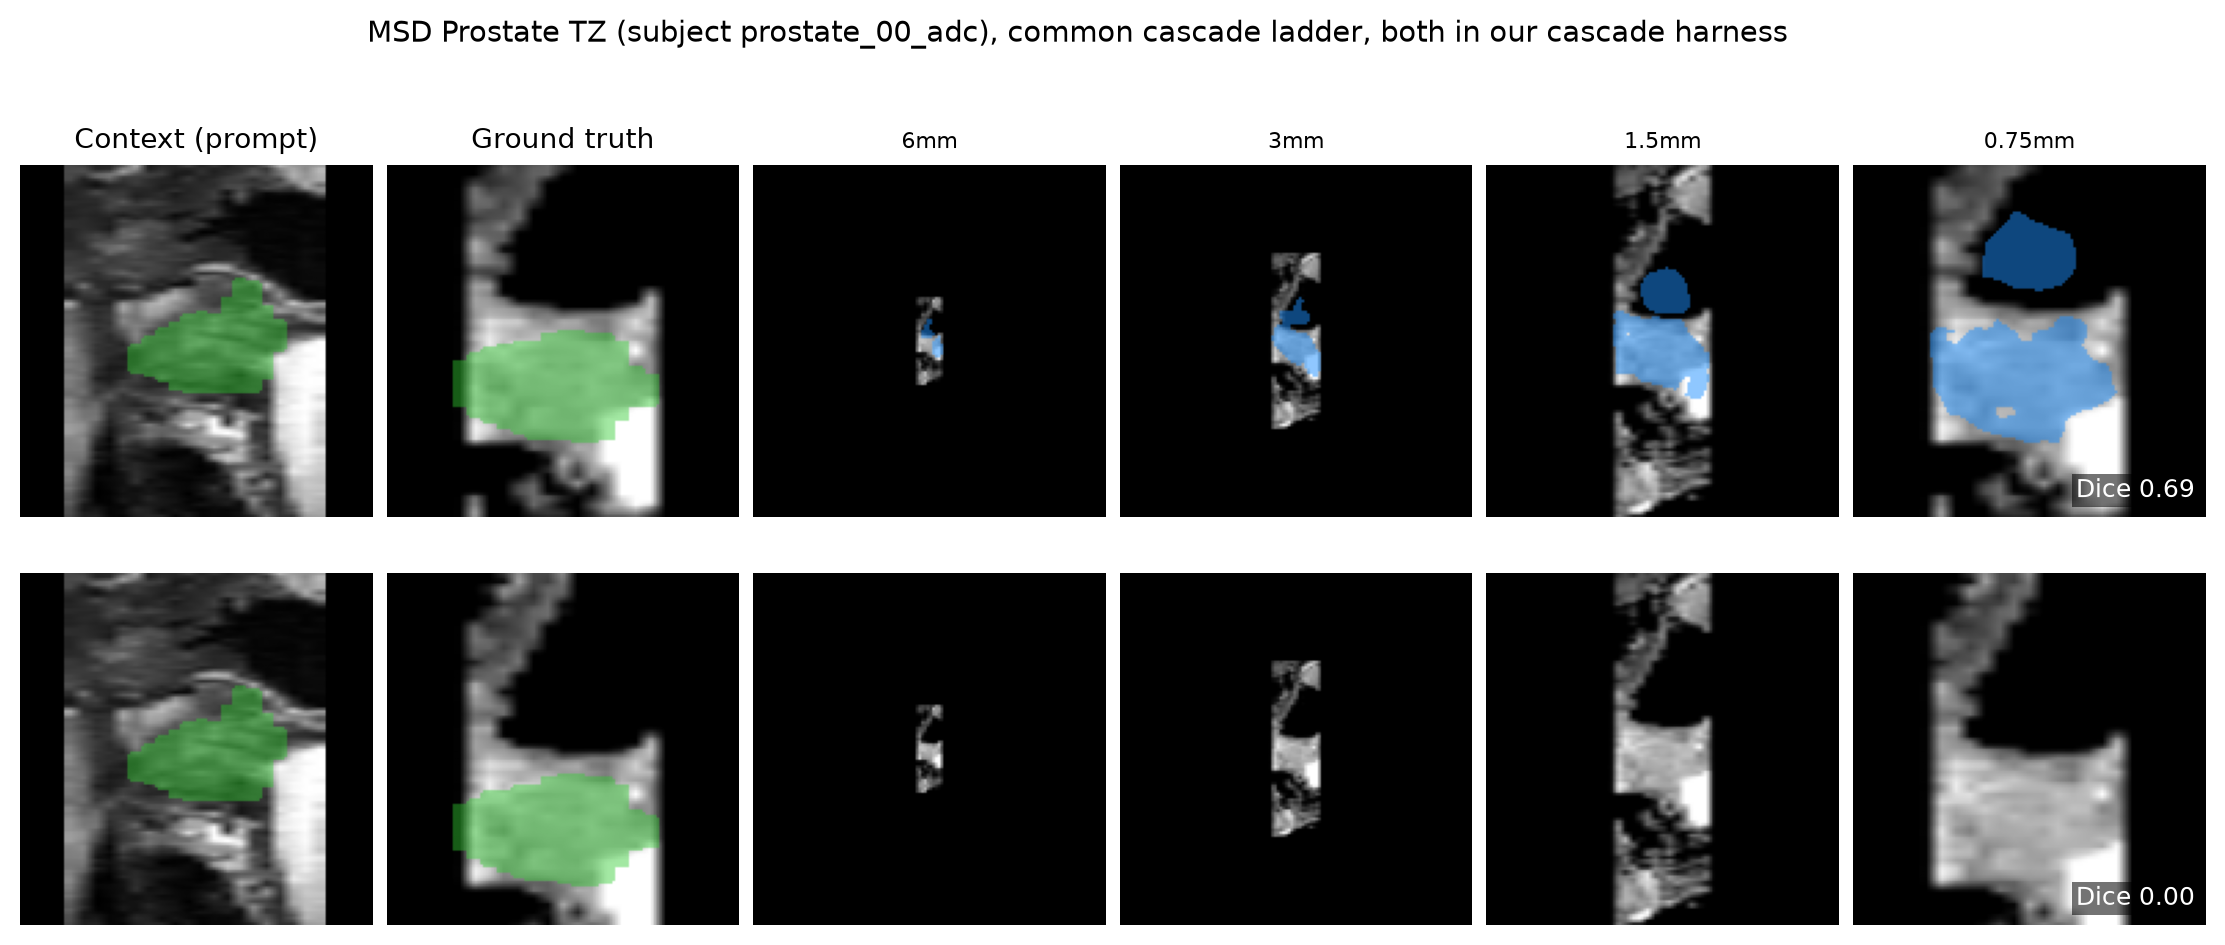
\includegraphics[width=\linewidth]{msd_prostate_cascade_win.png}
  \caption{MSD Prostate, TZ class, subject prostate\_00\_adc, common
  $[6,3,1.5,0.75]$\,mm ladder for both models: Cascade's prediction grows to
  fill the zone's shape while Medverse's stays empty at every level.}
  \label{fig:cascade-vs-medverse-cascade}
\end{figure}

\begin{figure}[t]
  \centering
  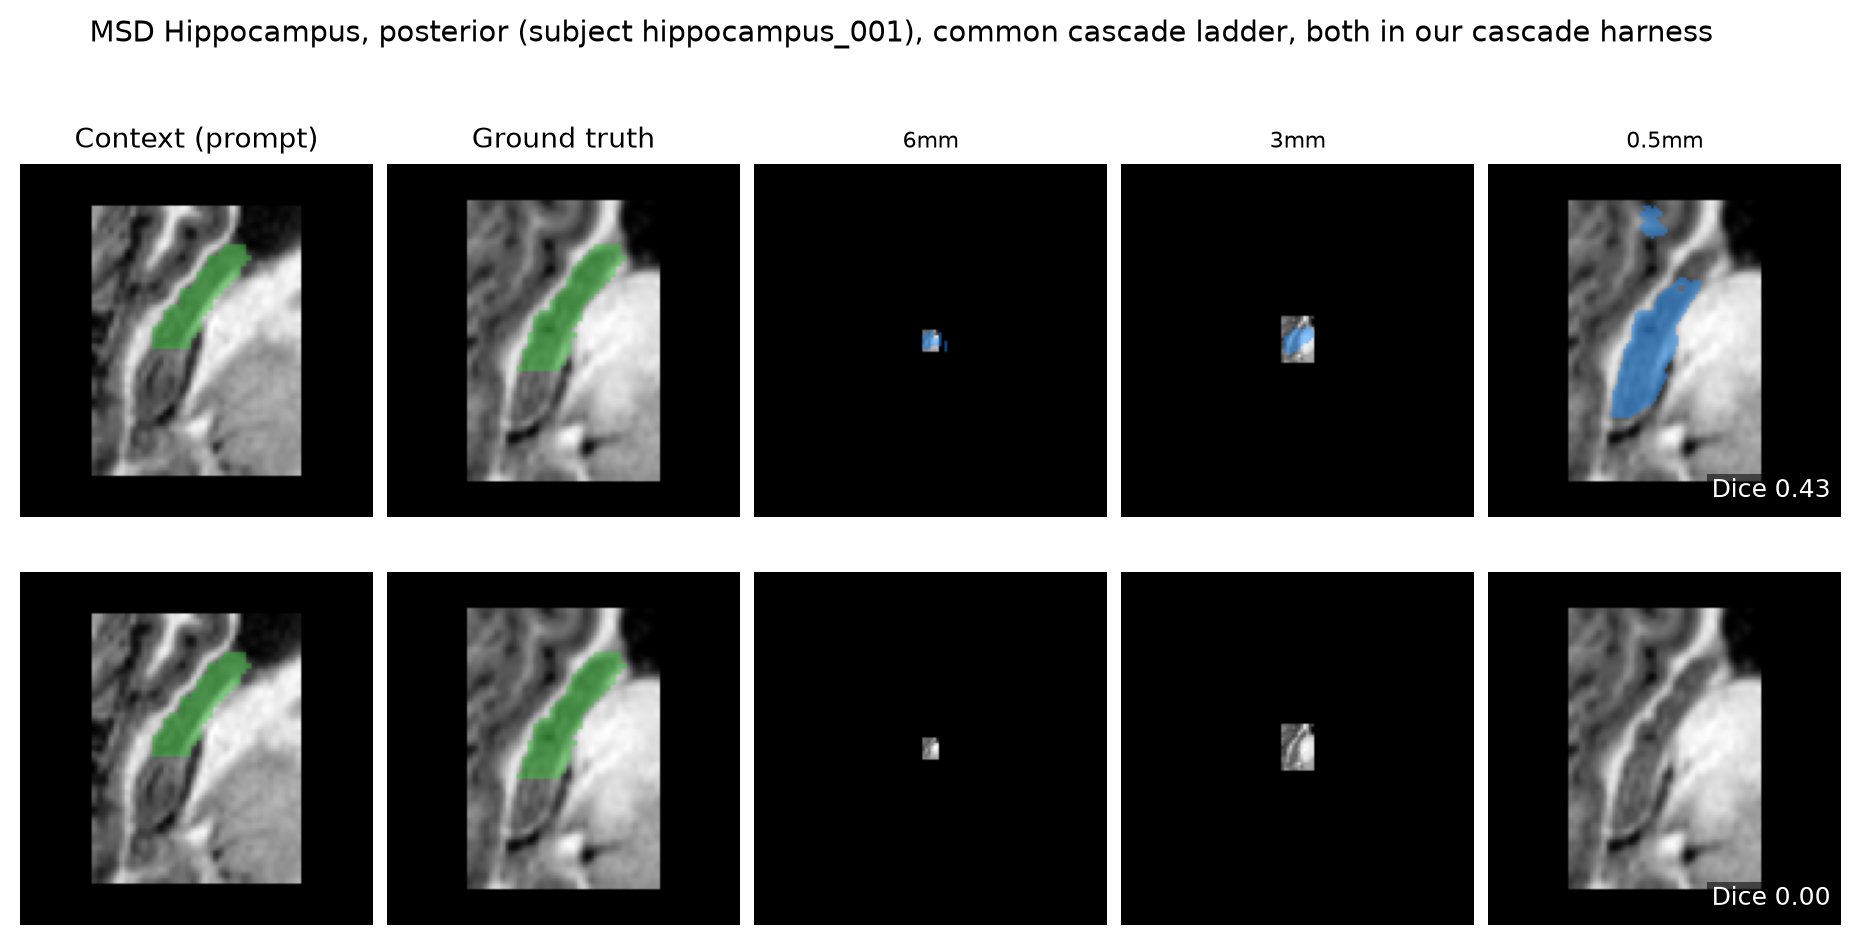
\includegraphics[width=\linewidth]{msd_hippocampus_cascade_prior_fail.png}
  \caption{MSD Hippocampus, posterior class, subject hippocampus\_001, common
  $[6,3,0.5]$\,mm ladder for both models: Medverse's box is placed correctly
  at every level but its prediction collapses to empty throughout, consistent
  with the aggregate drop from 0.691 (no prior) to 0.050 (prior) in
  \autoref{tab:medverse-prior-appendix}. Cascade's prediction, forced through
  the same 3-level ladder for this figure only, is fragmented but present at
  every level.}
  \label{fig:cascade-vs-medverse-cascade-hip}
\end{figure}

\begin{figure}[t]
  \centering
  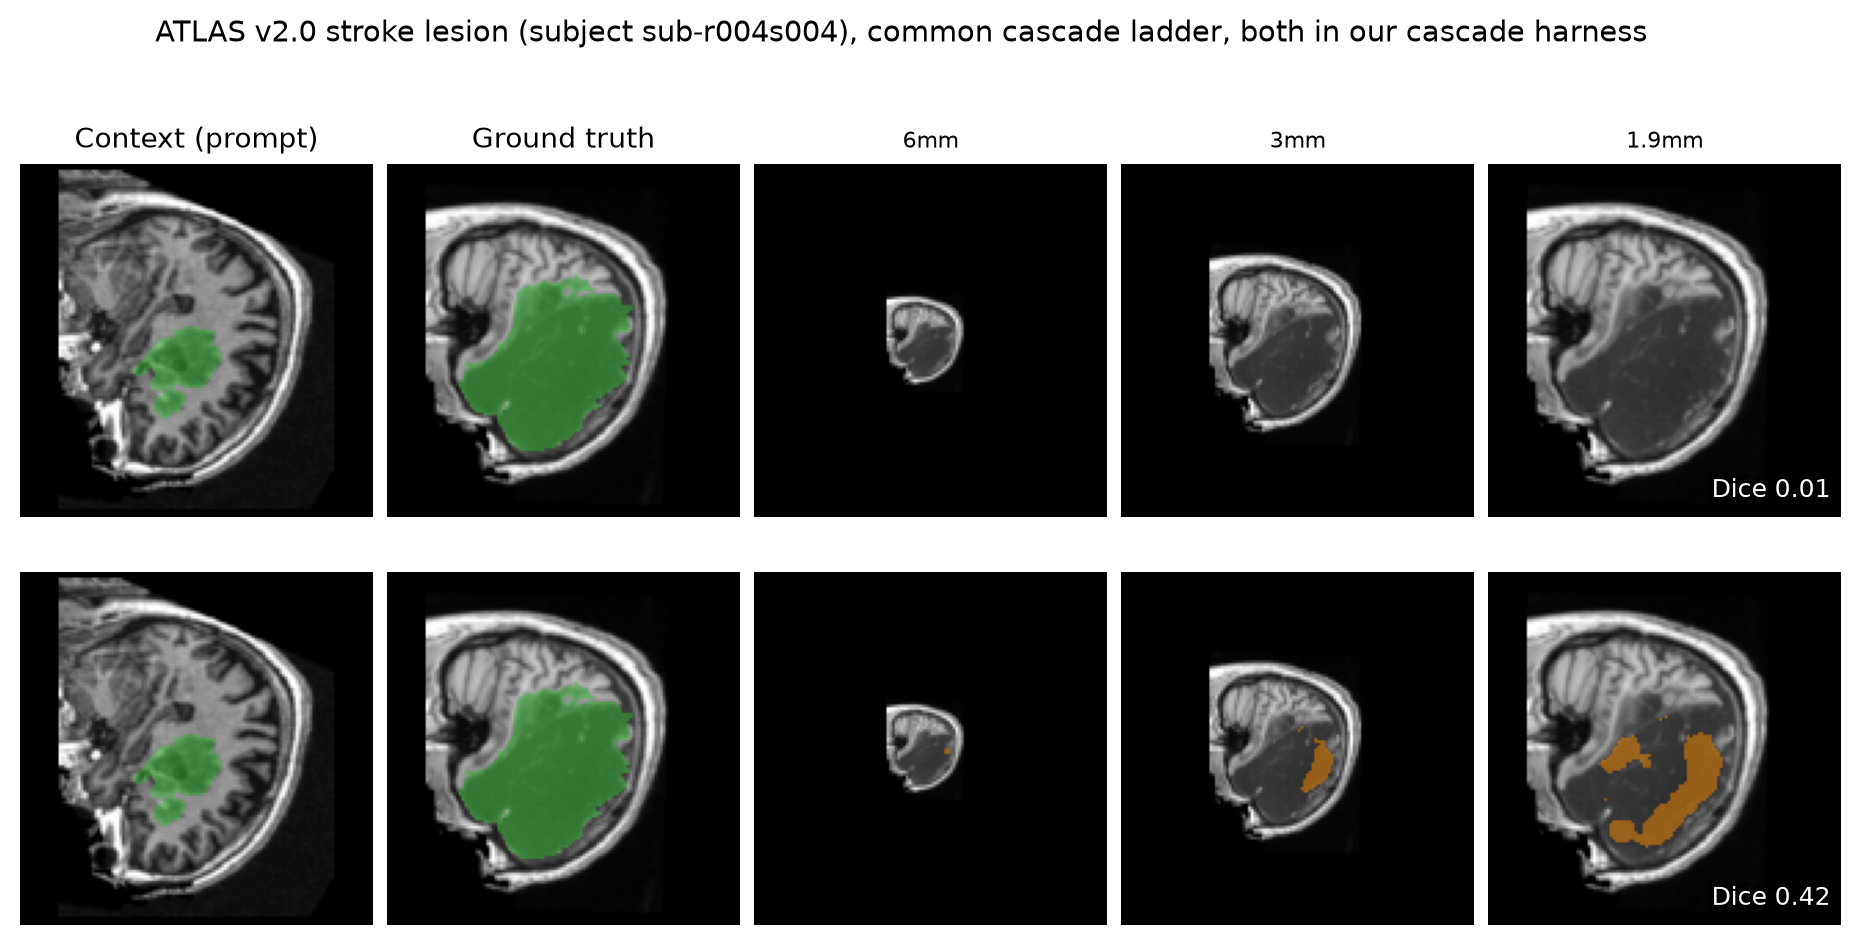
\includegraphics[width=\linewidth]{atlas_v2_cascade_medverse_win.png}
  \caption{ATLAS v2.0, stroke lesion, subject sub-r004s004, common
  $[6,3,1.9]$\,mm ladder for both models: Cascade's predicted region shrinks
  to almost nothing by its finest level while Medverse's prior-conditioned
  prediction grows to cover much of the lesion. This sample scores far above
  ATLAS v2.0's aggregate Prior Dice (0.42 vs.\ 0.020) and was chosen
  specifically to show that the prior does not hurt Medverse uniformly, not
  as a representative case.}
  \label{fig:cascade-vs-medverse-cascade-atlas}
\end{figure}
\todo[inline]{Single-sample illustrations, not aggregate-representative cases
(MSD Prostate's aggregate ``prior'' Dice is 0.251, not 0.00; the ATLAS v2.0
sample is an extreme outlier the other way, 0.42 vs.\ an aggregate of 0.020 --
both were picked to illustrate a pattern, not summarize the row). All three
panels are re-rendered directly from \texttt{cascade.run\_cascade} on these
specific (subject, context, class) triples -- not the harness's own saved
diagnostic panels -- so the color scheme is consistent (green GT / blue
Cascade / orange Medverse) and every level of a shared, common ladder is
shown for both models, not just the finest. Forcing Cascade onto a ladder it
was not evaluated on for the main tables (MSD Hippocampus's 3-level ladder;
ATLAS v2.0's $[6,3,1.9]$\,mm instead of $[3.8,1.9]$\,mm) changes its Dice from
the officially reported number (e.g.\ MSD Hippocampus 0.34$\to$0.43,
ATLAS v2.0 0.02$\to$0.01) -- expected since the crop geometry differs, but
worth being explicit that these two figures' Cascade numbers are not the ones
in \autoref{tab:cascade-medverse}. Checkpoints:
\texttt{2026-09-24\_146\_cascade\_randomfg\_predprior\_regoff/best.pt}
(Cascade, released weights for Medverse). The ATLAS v2.0 and common-ladder
(subject, context) pairs were not among the sources' saved figures at all and
required rerunning \texttt{run\_cascade} outside the full eval sweep;
Medverse's cascade-mode prediction on the ATLAS v2.0 sample is noticeably
unstable across reruns (0.42--0.88 Dice observed across otherwise-identical
reruns, plausibly bf16-autocast sensitivity compounding across its two
feedback steps) -- worth flagging as a finding in its own right, and reason
for caution reading any single Medverse-in-cascade number too precisely.}

\paragraph{Source of the label prior.}
\autoref{tab:cascade-ablation} compares two models that differ only in the
prior used during training: the model's own prediction from the previous
level, or a perturbed ground-truth mask. At inference, both use their own
predicted prior, since no ground truth is available then. On TotalSeg CT, the predicted prior is better on
99 of 117 classes (median difference $+0.043$ Dice) and also improves NSD
(0.631 vs.\ 0.576). MSD Hippocampus runs a single level, so no prior is
passed; its row reflects the two checkpoints, not the prior, and is excluded
from the counts below. On the remaining eight datasets outside the training
vocabulary (class-level held-out, \autoref{sec:results-setup}; this excludes
FLARE22 as well as TotalSeg CT), the predicted prior is better on five and
worse on three: Shifts-MS, ATLAS v2.0, and GNC\_705. These three, together with ISLES22, are lesion datasets
on which both priors score below 0.1; among these four, only ISLES22 favors
the predicted prior.

\begin{table}[t]
  \centering
  \small
  \caption{Macro Dice of models trained with a perturbed ground-truth prior or
  with their own predicted prior.}
  \label{tab:cascade-ablation}
  \begin{tabular}{@{}lcc@{}}
    \toprule
    Dataset & Perturbed ground truth & Predicted \\
    \midrule
    TotalSeg CT     & 0.543 & \textbf{0.586} \\
    TotalSeg MRI    & 0.449 & \textbf{0.506} \\
    FLARE22         & 0.731 & \textbf{0.751} \\
    MSD Prostate    & 0.310 & \textbf{0.375} \\
    MSD Hippocampus$^{*}$ & 0.319 & 0.303 \\
    HU\_LWK1        & 0.099 & \textbf{0.152} \\
    NasalSeg        & 0.399 & \textbf{0.547} \\
    \midrule
    ISLES22         & 0.067 & \textbf{0.069} \\
    Shifts-MS       & \textbf{0.035} & 0.031 \\
    ATLAS v2.0      & \textbf{0.029} & 0.026 \\
    GNC\_705        & \textbf{0.027} & 0.024 \\
    \bottomrule
  \end{tabular}
  \par\vspace{0.5em}
  \raggedright\footnotesize
  $^{*}$MSD Hippocampus runs a single level, so no prior is passed; this row
  reflects the two checkpoints, not the prior, and is excluded from the
  counts in the text.
\end{table}
\todo[inline]{Planned ablations: no prior at all, and no region restriction
(full-volume sliding window at fine levels, same checkpoint).}

\paragraph{Register carry.}
A variant that additionally carries the register tokens across levels was
tested against the same predicted-prior checkpoint, with a mixed effect on
the same nine datasets: it lowers Dice on six (most on MSD Prostate,
$-0.016$) and raises it on three (most on NasalSeg, $+0.061$, and MSD
Hippocampus, $+0.097$).% <<< end sections/results_cascade.tex
% >>> begin sections/results_synth.tex
\subsection{Synthetic Task Generation}\label{sec:results-synth}

This section evaluates the synthetic task generator, mainly on the four
lesion datasets it targets: ISLES22, Shifts-MS, ATLAS v2.0, and GNC\_705. They
are the most difficult evaluation datasets, since their targets are lesions on
MRI with no counterpart among the training classes. Under cascade inference,
the comparison widens to all nine held-out datasets used in
\autoref{sec:results-cascade}.

\paragraph{Synthetic-bank canvas.}
The baseline is the Synth configuration trained with $p_\text{synth} = 0.5$
and the synthetic-bank canvas. It reaches Dice between 0.008 and 0.082 on the
four datasets (\autoref{tab:synth-realhost-ood}). Changing the mix of shape
families or $p_\text{synth}$ with this canvas did not change these results
beyond run-to-run variation.   The bank's images are synthesized from label maps of CT scans, whereas all
  four target datasets are real MRI. This suggested that the canvas, rather
  than the variety of shapes, limits transfer.
\todo[inline]{Show the family-mix and $p_\text{synth}$ runs (appendix table)}

\paragraph{Real-host canvas.}
To test this, we continued training from the baseline checkpoint in two runs
that differ only in the canvas: the synthetic bank (stage 1) or real scans from TotalSegmentator (stage 2). Both use only the scatter-field family, with
the same $p_\text{synth}$ and training budget. The real canvas improves Dice on
three of the four datasets: ISLES22 from 0.045 to 0.098, Shifts-MS from 0.011
to 0.058, and GNC\_705 from 0.070 to 0.105. ATLAS v2.0 is unchanged (0.033
vs.\ 0.032). ATLAS v2.0 mostly contains single compact lesions, whereas
scatter-field shapes consist of many small components, which may explain why
it does not benefit. Absolute Dice remains low on all four datasets.
\todo[inline]{Confirm that stages 1 and 2 are continued from the baseline
checkpoint, and what distinguishes stage 1 from the baseline.}

In stage 3, the real-host canvas is extended to all seven shape families and to
all TotalSegmentator subjects (CT and MRI, all organs), and training runs
longer. This raises Dice on GNC\_705 to 0.223, while ISLES22, Shifts-MS, and ATLAS
v2.0 all drop slightly below their stage-2 values. Because stage 3 changes
three factors at once, the result cannot be attributed to any one of them.

\begin{table}[t]
  \centering
  \small
  \caption{Dice on the lesion datasets for successive synthetic-task
  configurations. Stages 1 and 2 differ only in the canvas. Stage 3 adds all
  shape families, all TotalSegmentator subjects as canvas, and a longer
  training budget. Bold marks each dataset's best value across the four
  configurations, not the winner of any single stage-to-stage comparison
  (contrast \autoref{tab:synth-cascade-realhost}, where bold marks the best
  model per row).}
  \label{tab:synth-realhost-ood}
  \begin{tabular}{@{}lcccc@{}}
    \toprule
    Configuration & ISLES22 & Shifts-MS & ATLAS v2.0 & GNC\_705 \\
    \midrule
    Baseline                          & 0.050 & 0.008 & 0.028 & 0.082 \\
    1) Synthetic bank, scatter field  & 0.045 & 0.011 & \textbf{0.033} & 0.070 \\
    2) Real host, scatter field       & \textbf{0.098} & \textbf{0.058} & 0.032 & 0.105 \\
    3) Real host, all families        & 0.087 & 0.051 & 0.027 & \textbf{0.223} \\
    \bottomrule
  \end{tabular}
\end{table}

\paragraph{Effect on TotalSegmentator.}
\autoref{tab:synth-realhost-indist} reports TotalSegmentator validation Dice
for the same checkpoints. Stages 1 and 2 change it by at most 0.012 in any
column, so the gains of stage 2 on the lesion datasets do not reduce accuracy
on the training distribution. Stage 3 improves all five values, from 0.418 to
0.490 overall. Given its longer training budget, this gain likely reflects the
additional training rather than the synthetic tasks themselves.

\begin{table}[t]
  \centering
  \small
  \caption{TotalSegmentator validation Dice for the checkpoints of
  \autoref{tab:synth-realhost-ood}, overall, by class membership (seen,
  unseen), and by modality (MRI, CT).}
  \label{tab:synth-realhost-indist}
  \begin{tabular}{@{}lccccc@{}}
    \toprule
    Configuration & All & Seen & Unseen & MRI & CT \\
    \midrule
    Baseline                          & 0.418 & 0.489 & 0.344 & 0.390 & 0.468 \\
    1) Synthetic bank, scatter field  & 0.422 & 0.485 & 0.356 & 0.385 & 0.470 \\
    2) Real host, scatter field       & 0.417 & 0.483 & 0.348 & 0.384 & 0.467 \\
    3) Real host, all families        & \textbf{0.490} & \textbf{0.579} & \textbf{0.397} & \textbf{0.474} & \textbf{0.534} \\
    \bottomrule
  \end{tabular}
\end{table}

\paragraph{Cascade inference.}
Synth + Cascade continues the stage-3 checkpoint with 20 epochs of cascade
training. \autoref{tab:synth-cascade-realhost} compares it with Cascade, which
uses no synthetic tasks, and with step-matched Medverse on the nine held-out
datasets. Synth + Cascade improves on MSD Hippocampus (0.303 to 0.518) and
NasalSeg (0.547 to 0.644), is worse on HU\_LWK1 ($-0.028$) and Shifts-MS
($-0.012$), and differs by at most 0.011 on the other datasets. It remains
below Medverse on MSD Hippocampus and NasalSeg. The two models differ in more
than the synthetic tasks: Synth + Cascade also uses register carry and a
pooling token, and has a different training history. The differences can
therefore not be attributed to the synthetic tasks alone.

\begin{table}[t]
  \centering
  \small
  \caption{Dice on the held-out datasets under cascade inference. Medverse:
  released weights, step-matched autoregressive inference
  (\autoref{sec:results-cascade}); omitted where both models score too low to
  be informative. Cascade and Synth + Cascade use the same per-dataset ladder
  (identical sample counts confirmed for every dataset), so differences are
  not a ladder confound; Medverse uses its own depth-matched ladder from
  \autoref{tab:cascade-medverse}.}
  \label{tab:synth-cascade-realhost}
  \begin{tabular}{@{}lcccc@{}}
    \toprule
    Dataset & Spacings (mm) & Cascade & Synth + Cascade & Medverse \\
    \midrule
    HU\_LWK1        & $[6, 3, 1]$      & \textbf{0.152} & 0.124 & 0.020 \\
    ISLES22         & $[3, 1.5]$       & 0.069 & \textbf{0.070} & -- \\
    Shifts-MS       & $[3, 1.5]$       & \textbf{0.031} & 0.019 & -- \\
    ATLAS v2.0      & $[3.8, 1.9]$     & 0.026 & \textbf{0.032} & -- \\
    MSD Prostate    & $[3, 1.5, 0.75]$ & \textbf{0.375} & 0.372 & 0.357 \\
    MSD Hippocampus & $[0.5]$          & 0.303 & 0.518 & \textbf{0.686} \\
    GNC\_705        & $[6, 3, 1.2]$    & 0.024 & \textbf{0.035} & -- \\
    FLARE22         & $[6, 3, 2.5]$    & \textbf{0.751} & 0.743 & 0.359 \\
    NasalSeg        & $[1.5, 0.8]$     & 0.547 & 0.644 & \textbf{0.737} \\
    \bottomrule
  \end{tabular}
\end{table}

The gain on GNC\_705 at a single level (0.223,
\autoref{tab:synth-realhost-ood}) does not carry over to cascade inference,
where both models score below 0.04. A likely cause is localization: on this
dataset, the coarse predictions follow bright regions rather than the lesions,
so the region-restricted fine levels process crops that miss the lesion. This
illustrates the limitation of region restriction noted in
\autoref{sec:methodology-cascade}: small targets that the coarse level
mislocalizes cannot be recovered. \autoref{fig:gnc-localization-fail} shows one
such case: the lesion is a handful of voxels at the edge of the kidney
(yellow circle, added for visibility, on the ground-truth panel), and the
region-restricted finest level predicts nothing in that same location
(Dice 0.00).

\begin{figure}[t]
  \centering
  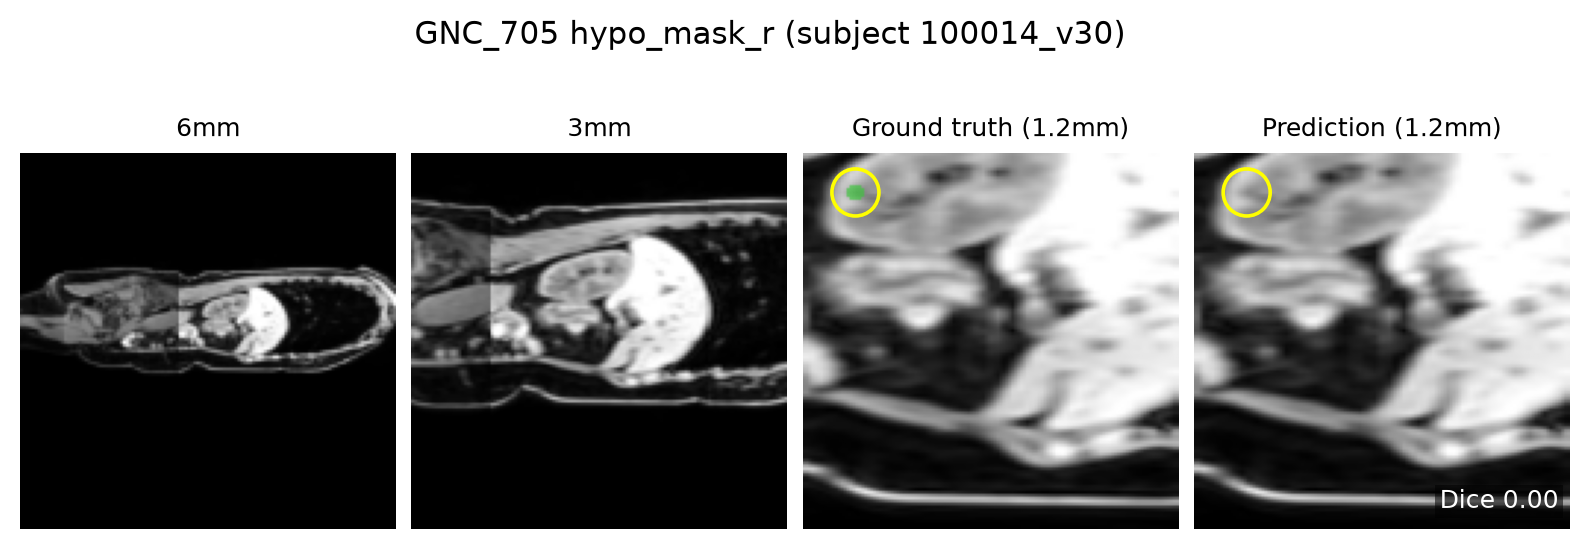
\includegraphics[width=\linewidth]{gnc_localization_fail.png}
  \caption{GNC\_705, class hypo\_mask\_r, subject 100014\_v30 (Cascade
  checkpoint), coarse (6\,mm) and mid (3\,mm) level images shown for context:
  the lesion (yellow circle) is a handful of voxels at the edge of the
  kidney; the finest (1.2\,mm) level, restricted to its own region, predicts
  nothing there (Dice 0.00).}
  \label{fig:gnc-localization-fail}
\end{figure}
\todo[inline]{Support this further with the containment of the coarse box on
GNC\_705 across all samples, not just this one case (currently a single
qualitative example, re-rendered directly from \texttt{cascade.run\_cascade}
on this one (subject, context, class) triple, not a systematic worst-case
search), instead of the reference to
\texttt{docs/datasets/gnc\_kidney\_lesions.md}. If the single-level evaluation
uses ground-truth-centered crops, the drop may mainly reflect the loss of
ground-truth localization; state which is the case.}

% <<< end sections/results_synth.tex
% <<< end sections/results.tex
% >>> begin sections/discussion.tex
\section{\iflanguage{english}{Discussion}{Diskussion}}\label{sec:discussion}

This chapter summarizes what the experiments show for each of the three
questions raised in \autoref{sec:motivation}, discusses the limitations of the
evidence, and outlines open questions.

\subsection{Image--Label Fusion}\label{sec:discussion-fusion}

Replacing Medverse's two U-Nets with a shared encoder and attention layers
improved accuracy on classes from the training vocabulary by a large margin,
between 0.16 and 0.23 Dice on TotalSegmentator and FLARE22
(\autoref{tab:fusion-staircase}). On new targets, this change alone did not
help: early fusion was below Dual U-Net Cross-Attn on MSD Prostate, MSD
Hippocampus, and HU\_LWK1. Dual attention changed this pattern only partly.
Its gains over early fusion were small on in-vocabulary classes and larger on
new targets and on the unseen modality, and it was the only variant above Dual
U-Net Cross-Attn on the sample-weighted mean over held-out sources. This
aggregate advantage does not hold source-by-source: on the five lesion and
cavity datasets, Dual U-Net Cross-Attn wins more often (four of five), so the
mean is driven by the first five, more anatomical, held-out sources.

One interpretation is that repeated interaction between image and label tokens
matters most when the model cannot rely on having seen the class during
training and has to extract the target from the context masks. This is
consistent with the results, but they do not test it directly. Dual attention
also remained well below Dual U-Net Cross-Attn on MSD Prostate and HU\_LWK1.
Dual U-Net Cross-Attn starts from Medverse's weights, which were trained on
different data; part of its advantage on these datasets may come from that
pretraining rather than from its architecture.

Dual attention reached these results with the fewest parameters of the three
variants. The GFLOPs of the three variants differ by up to 65\%, but their
latency is nearly identical, so GFLOPs did not predict latency in this
setting.
\todo[inline]{Check where the time goes (e.g.\ encoder, data movement) before
drawing conclusions about compute.}

\subsection{Coarse-to-Fine Cascade}\label{sec:discussion-cascade}

When each level's crop is placed from the previous level's prediction, Dice
still increases from level to level on every dataset
(\autoref{tab:cascade-levels}). On TotalSeg CT, the coarse level localizes the
target well enough for the first, coarsest-to-middle step: a box at its
predicted centroid contains 92\% of the target's voxels on average, compared
with 97\% for a box at the ground-truth centroid, and most of the remaining
error at this step arises within the fine crops rather than from
localization; the middle-to-finest step is not measured this way.

The clearest advantage over Medverse is speed. Cascade is about 14 times faster
than Medverse with the same number of refinement steps. The accuracy comparison
depends on how Medverse is run. With matched steps, Cascade is more accurate on
five of seven datasets; against Medverse at its native number of steps, it is
more accurate on five of the nine datasets where a native run exists (FLARE22,
HU\_LWK1, ISLES22, ATLAS v2.0, and GNC\_705). The efficiency result is thus
better supported than the accuracy result, and the accuracy comparison on
TotalSegmentator additionally depends on verifying Medverse's low scores
there.

Training with the model's own predictions as prior worked better than training
with perturbed ground-truth masks on the training distribution (99 of 117
classes) and was mixed on datasets outside the training vocabulary (five of
eight). A plausible
explanation is that a model trained on its own predictions sees, during
training, the kind of errors it will encounter at inference, which a
hand-designed perturbation of the ground truth only approximates. Whether the
prior helps at all compared with no prior has not been tested yet. The
experiment with Medverse inside our cascade shows that a prior can also hurt:
passing Medverse's coarse prediction forward lowered its Dice on six of seven
datasets.

Region restriction makes the cost of the fine levels depend on the size of the
target rather than the size of the volume, but it makes the fine levels depend
on the coarse localization. GNC\_705 shows the consequence: its single-level
Dice of 0.223 dropped below 0.04 under cascade inference, likely because the
coarse level mislocalizes the small lesions. Small, multi-focal, or low-contrast
targets are the cases where this failure is most likely. Possible remedies
include larger margins, several boxes per volume for multi-focal targets, or
falling back to full-volume processing when the coarse prediction is uncertain.
\todo[inline]{Revise the GNC\_705 paragraph once it is clear whether the
single-level evaluation used ground-truth-centered crops
(\autoref{sec:results-synth}).}

\subsection{Synthetic Task Generation}\label{sec:discussion-synth}

With the synthetic-bank canvas, varying the shapes and the fraction of
synthetic tasks had no measurable effect on the lesion datasets. Changing only
the canvas from CT bank images to real MRI cases improved three of four lesion
datasets without reducing accuracy on TotalSegmentator. This indicates that
the image the shapes are painted on mattered more than the variety of shapes,
at least when the canvas and the target data differ in modality.

The effect of synthetic tasks under cascade inference was smaller and
different. Synth + Cascade improved mainly on MSD Hippocampus and NasalSeg,
which are anatomical structures rather than lesions, and not on the lesion
datasets that motivated the generator. Since Synth + Cascade also differs from
Cascade in other components and in training history, these gains cannot be
attributed to the synthetic tasks alone.

Across all configurations, Dice on the lesion datasets stayed low: at most
0.223 at a single level and below 0.08 under cascade inference. In-context
segmentation of lesions remains largely unsolved in this setting. Lesions vary
in location, number, and shape far more than anatomical structures, so the
context examples say less about where the target is. How much of this gap
synthetic tasks can close remains open.

\subsection{Limitations}\label{sec:discussion-limitations}

\paragraph{Strength of the evidence.}
All results come from a single training run per configuration, so no variance
estimates are available, and differences of a few hundredths of Dice should not
be over-interpreted. Several results rest on few classes, such as the two
unseen FLARE22 classes, the MSD datasets with two classes each, and HU\_LWK1
with one. In the fusion comparison, early fusion and dual attention had not
completed their training budget, while Dual U-Net Cross-Attn had converged.

\paragraph{Differences between configurations.}
The three results sections use different model configurations
(\autoref{tab:configs}), so their numbers cannot be compared with each other.
Within sections, some comparisons change several factors at once: stage 3 of
the synthetic-task experiments changes shape families, canvas pool, and
training budget together, and Synth + Cascade differs from Cascade in more than
the synthetic tasks.
\todo[inline]{Update if a single final configuration is evaluated before
submission.}

\paragraph{Missing ablations.}
The contribution of the label prior and of region restriction has not been
isolated: the cascade has not been evaluated without a prior or with
full-volume processing at the fine levels. The speedup over Medverse therefore
reflects the whole system, not region restriction alone.

\paragraph{Baselines and data.}
Medverse is the only baseline evaluated empirically. Iris and UniverSeg are
compared only by design. The overlap between Medverse's training data and our
evaluation datasets is not fully documented, which affects the comparison on
TotalSegmentator, MSD Hippocampus, and NasalSeg. The provenance of the ATLAS
v2.0 copy used here has not been confirmed.
\todo[inline]{Remove the ATLAS sentence once provenance is confirmed or the
dataset is dropped.}

\subsection{Open Questions}\label{sec:discussion-open}

The most direct next steps are the missing ablations (no prior, no region
restriction), additional seeds, and a single final configuration evaluated on
all datasets. Beyond these, three questions remain open. First, the position
axis attends over the tokens of all $K+1$ volumes at once, so its cost grows
quadratically with the number of context volumes. How accuracy and cost scale
with $K$ has not been studied. Second, region restriction needs a way to
handle targets the coarse level cannot localize reliably. Third, synthetic
tasks helped on some held-out datasets, but not yet on lesions under cascade
inference. Generating tasks that resemble lesions in appearance and
distribution, not only in shape, is one direction to explore.% <<< end sections/discussion.tex
% >>> begin sections/conclusion.tex
\section{\iflanguage{english}{Conclusion}{Fazit}}\label{sec:conclusion}

This thesis studied in-context segmentation of 3D medical images and addressed
three questions: how to combine image and label information, where to spend
compute, and how to obtain training data beyond the annotated classes.

For the first question, we proposed dual attention, which keeps image and label
tokens separate and lets them interact in every layer. In a comparison trained
on TotalSegmentator CT, dual attention improved over merging the two once,
mainly on new targets and on an unseen modality, and it did so with the fewest
parameters of the compared variants. It was also the only shared-encoder
variant above a retrained Medverse architecture on the mean over held-out
datasets, although not on every dataset.

For the second question, we proposed a coarse-to-fine cascade in which each
level receives the previous level's prediction as a prior and processes only
the region that prediction localizes. The cascade was about 14 times faster
than Medverse with the same number of refinement steps. It was more accurate
than step-matched Medverse on five of seven datasets, but the comparison with
Medverse at its native depth was mixed. Training with the model's own
predictions as prior worked better than training with perturbed ground-truth
masks on the training distribution.

For the third question, we proposed a synthetic task generator that paints
procedural shapes onto scans. The modality of the image the shapes are painted
on mattered more than the variety of shapes: painting onto real MRI cases
improved three of four lesion datasets at a single level without reducing
accuracy on TotalSegmentator. Under cascade inference, synthetic tasks helped
on held-out anatomical structures but not on lesions.

All results come from single training runs, and several comparisons are not
fully controlled; \autoref{sec:discussion-limitations} lists the main
limitations and the ablations still missing. Segmenting lesions from a few
examples remains the hardest case in this setting and the clearest direction
for future work.
\todo[inline]{Update the numbers and claims once the pending re-runs and
ablations are complete.}% <<< end sections/conclusion.tex

\pagenumbering{Roman}
% >>> begin sections/symbols.tex
% Choose a style, e.g. here:
% https://www.dickimaw-books.com/gallery/glossaries-styles/
\printglossary[type=symbols,style=long-name-desc-loc]
% <<< end sections/symbols.tex
% >>> begin sections/figures.tex
\listoffigures
% <<< end sections/figures.tex
% >>> begin sections/tables.tex
\listoftables
% <<< end sections/tables.tex
% >>> begin sections/algorithms.tex
\renewcommand{\lstlistlistingname}{\iflanguage{english}{List of Algorithms}{Algorithmenverzeichnis}}
\addcontentsline{toc}{section}{\iflanguage{english}{List of Algorithms}{Algorithmenverzeichnis}}
\lstlistoflistings
% <<< end sections/algorithms.tex
% >>> begin sections/glossary.tex
% Choose a style, e.g. here:
% https://www.dickimaw-books.com/gallery/glossaries-styles/
\printglossary[type=main,style=long-name-desc-loc]
% <<< end sections/glossary.tex
% >>> begin sections/references.tex
\bibliographystyle{plain}
\bibliography{references/motivation,references/fundamentals}
% <<< end sections/references.tex
% >>> begin sections/appendix.tex
\addcontentsline{toc}{section}{\iflanguage{english}{Appendix}{Anhang}}
\section*{\iflanguage{english}{Appendix}{Anhang}}\label{sec:appendix}

\begin{figure}[t]
  \centering
  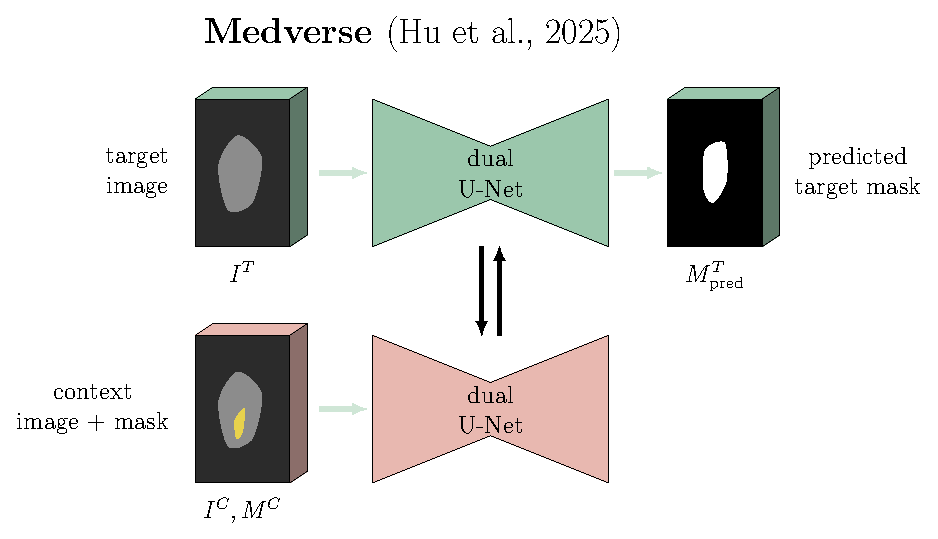
\includegraphics[width=0.6\linewidth]{arch_medverse.pdf}
  \caption{Medverse's architecture: dual U-Net cross-attention, shown for comparison against our architecture (\autoref{fig:overview}).}
  \label{fig:overview-medverse}
\end{figure}

\begin{table}[p]
  \centering
  \small
  \caption{TotalSegmentator classes used for training (seen) and held out
  (unseen), with the number of classes per category in parentheses.
  $^\dagger$: also available on TotalSegmentator MRI. On MRI, 50 classes are
  available, 31 of them seen.}
  \label{tab:totalseg-classes}
  \begin{tabularx}{\linewidth}{@{}p{3.2cm}XX@{}}
    \toprule
    Category & Seen & Unseen \\
    \midrule
    Organs, abdomen and pelvis (12\,/\,5)
      & adrenal gland L$^\dagger$, colon$^\dagger$, duodenum$^\dagger$,
        esophagus$^\dagger$, gallbladder$^\dagger$, kidney L$^\dagger$,
        liver$^\dagger$, pancreas$^\dagger$, small bowel$^\dagger$,
        spleen$^\dagger$, stomach$^\dagger$, urinary bladder$^\dagger$
      & adrenal gland R$^\dagger$, kidney R$^\dagger$, prostate$^\dagger$,
        kidney cyst L, kidney cyst R \\
    \addlinespace
    Organs, thorax, head, and spine (8\,/\,3)
      & brain$^\dagger$, heart$^\dagger$, spinal cord$^\dagger$, thyroid
        gland, trachea, lung lower lobe L, lung middle lobe R, lung upper
        lobe R
      & lung lower lobe R, lung upper lobe L, left atrial appendage \\
    \addlinespace
    Muscles (5\,/\,5)
      & autochthon L$^\dagger$, gluteus maximus L$^\dagger$, gluteus medius
        R$^\dagger$, gluteus minimus L$^\dagger$, iliopsoas R$^\dagger$
      & autochthon R$^\dagger$, gluteus maximus R$^\dagger$, gluteus medius
        L$^\dagger$, gluteus minimus R$^\dagger$, iliopsoas L$^\dagger$ \\
    \addlinespace
    Bones, limbs, shoulder, and pelvis (6\,/\,5)
      & clavicle R$^\dagger$, femur L$^\dagger$, hip R$^\dagger$, humerus
        L$^\dagger$, scapula L$^\dagger$, skull
      & clavicle L$^\dagger$, femur R$^\dagger$, hip L$^\dagger$, humerus
        R$^\dagger$, scapula R$^\dagger$ \\
    \addlinespace
    Bones, spine (11\,/\,15)
      & sacrum$^\dagger$; vertebrae C3, C7, T3, T6, T9, T12, L1, L3, L5, S1
      & vertebrae C1, C2, C4--C6, T1, T2, T4, T5, T7, T8, T10, T11, L2, L4 \\
    \addlinespace
    Bones, ribs and sternum (9\,/\,17)
      & sternum, costal cartilages; ribs L2, L3, L9, L12, R2, R6, R11
      & ribs L1, L4--L8, L10, L11, R1, R3--R5, R7--R10, R12 \\
    \addlinespace
    Vessels (10\,/\,6)
      & aorta$^\dagger$, inferior vena cava$^\dagger$, portal and splenic
        vein$^\dagger$, iliac artery L$^\dagger$, iliac vein L$^\dagger$,
        superior vena cava, pulmonary vein, brachiocephalic trunk, common
        carotid artery L, subclavian artery L
      & iliac artery R$^\dagger$, iliac vein R$^\dagger$, common carotid
        artery R, subclavian artery R, brachiocephalic vein L,
        brachiocephalic vein R \\
    \midrule
    MRI only (0\,/\,4)
      & --
      & lung L, lung R, vertebrae (all levels merged), intervertebral discs \\
    \bottomrule
  \end{tabularx}
\end{table}

\begin{table}[t]
  \centering
  \small
  \caption{Medverse's released weights run inside our cascade inference
  (\autoref{sec:results-cascade}, ``Medverse with our cascade''), with and
  without its own coarse prediction passed forward as a prior. Macro Dice.}
  \label{tab:medverse-prior-appendix}
  \begin{tabular}{@{}lcc@{}}
    \toprule
    Dataset & No prior & Prior \\
    \midrule
    HU\_LWK1        & 0.000 & 0.000 \\
    ISLES22         & 0.049 & 0.035 \\
    Shifts-MS       & 0.036 & 0.028 \\
    MSD Hippocampus & 0.691 & 0.050 \\
    MSD Prostate    & 0.327 & 0.251 \\
    ATLAS v2.0      & 0.126 & 0.020 \\
    GNC\_705        & 0.008 & 0.001 \\
    \bottomrule
  \end{tabular}
\end{table}% <<< end sections/appendix.tex

\end{document}
